% -----------------------------------------------------------------
% => RELATED WORKS
% -----------------------------------------------------------------

\chapter{Trabalhos Correlatos} \label{Chap:relatedWork}

% Este capítulo apresenta e discute os principais trabalhos existentes na literatura e que se relacionam com esta proposta de Tese. Por essa razão, as pesquisas abordadas a seguir são propostas de desenvolvimento de ambientes de sala de aula com inserção de novas tecnologias, isto é, ambientes de sala de aula inteligente (do inglês, \textit{smart classroom}). Além disso, são apresentados também trabalhos relacionados a autoria de objetos de aprendizagem e avaliação do desempenho dos estudantes em aulas apoiadas por tecnologia.

Este capítulo apresenta e discute os principais trabalhos existentes na literatura e que se relacionam com esta Tese. Por essa razão, as pesquisas abordadas a seguir são propostas de utilização de sistemas ciberfísicos no contexto educacional (Seção~\ref{sec:ciberfisicos}). Além disso, a integração desses sistemas ao processo educacional como um todo, isto é, ao planejamento, execução e avaliação do ensino-aprendizagem implica não apenas na construção de objetos de aprendizagem que sejam tangíveis (físico-digitais), mas, ainda, na necessidade de ferramentas de autoria e utilização desses objetos (Seção~\ref{sec:autoria}), além de ferramentas de avaliação da aprendizagem dos estudantes em aulas apoiadas por tecnologia (Seção~\ref{sec:avaliacao}).

\section{Sistemas Ciberfísicos na Educação}
\label{sec:ciberfisicos}

%O uso de sistemas ciberfísicos no contexto educacional tem sido objeto de diversas pesquisas nos últimos anos, onde alguns estudos apenas implementam manipulativos físicos e virtuais em separado com a finalidade de realizar comparações~\citep{zacharia:2011, Salehi:2014}, outros trabalhos mais recentes utilizam manipulativos híbridos (físico-virtuais)~\citep{ha:2018, Azad:2016} ou utilizam físicos e virtuais concomitantemente~\citep{Blikstein:2012, Blikstein2016}. De modo geral, o que se tem notado é que a associação entre o físico e o virtual tende a ajudar mais os processos de aprendizagem dos estudantes do que a utilização exclusiva de apenas um tipo de manipulativo. %Além disso, apenas o trabalho de~\cite{Santos:2014} foi encontrado em publicações vinculadas ao Congresso Brasileiro de Informática na Educação (CBIE).

O uso de manipulativos no contexto educacional tem sido objeto de diversas pesquisas nos últimos anos, onde alguns estudos investigam o uso de manipulativos físicos e virtuais em separado com a finalidade de realizar comparações~\citep{zacharia:2011, Salehi:2014}, outros trabalhos mais recentes utilizam manipulativos tangíveis (físico-digitais)~\citep{ha:2018, Azad:2016} ou utilizam físicos e virtuais concomitantemente~\citep{Blikstein:2012, Blikstein2016}. De modo geral, o que se tem notado é que a associação entre o físico e o virtual tende a ajudar mais os processos de aprendizagem dos estudantes do que a utilização exclusiva de apenas um tipo de manipulativo. %Além disso, apenas o trabalho de~\cite{Santos:2014} foi encontrado em publicações vinculadas ao Congresso Brasileiro de Informática na Educação (CBIE).

Antes de prosseguirmos, é importante salientar que, neste texto, o termo Manipulativo Virtual (MV) refere-se ``a visualizações dinâmicas virtuais interativas de aparelhos e materiais, fornecidas por meio de uma simulação computacional (laboratório virtual)'', conforme apresentado por \cite{zacharia:2011}, de modo que a experiência de aprendizagem acontece através da interação/manipulação de um material totalmente virtual que simula o mundo físico. Além disso, Manipulativo Físico (MF) é um objeto de aprendizagem de interação manual sem qualquer nível de conectividade computacional e Manipulativo Tangível (ou físico-digital) corresponde aos objetos apresentados na seção~\ref{section:TUI}.

\subsection{Manipulativos Físicos \textit{versus} Manipulativos Virtuais}

\textbf{Aprendizado de Física}\\
~\cite{zacharia:2011} realizaram experimentos para comparar se a utilização de manipulativos físicos (MF) e virtuais (MV) tem algum diferencial no aprendizado de Física no Ensino Superior. Os experimentos são realizados em quatro cenários: (i) apenas MF; (ii) apenas MV; (iii) MF precedendo MV e; (iv) MV precedendo MF. Além disso, os efeitos da manipulação física ou virtual na compreensão dos estudantes acerca dos conceitos de calor e temperatura foram examinados e comparados a educação tradicional (modo passivo de instrução).

Para a condução dos experimentos, foi utilizado um laboratório real de física para o experimento com MF e o \textit{software ``Virtual Lab ThermoLab''} (Figura~\ref{fig:zacharia_thermolab}) para o experimento com MV. Participaram do estudo 234 universitários inscritos em um curso introdutório de física, sendo 55 do sexo masculino e 168 do sexo feminino e tendo uma média de idade de 18.5 anos. Estes estudantes foram divididos em grupos menores de acordo com os cenários já mencionados.

\begin{figure}[htb]
	\centering
	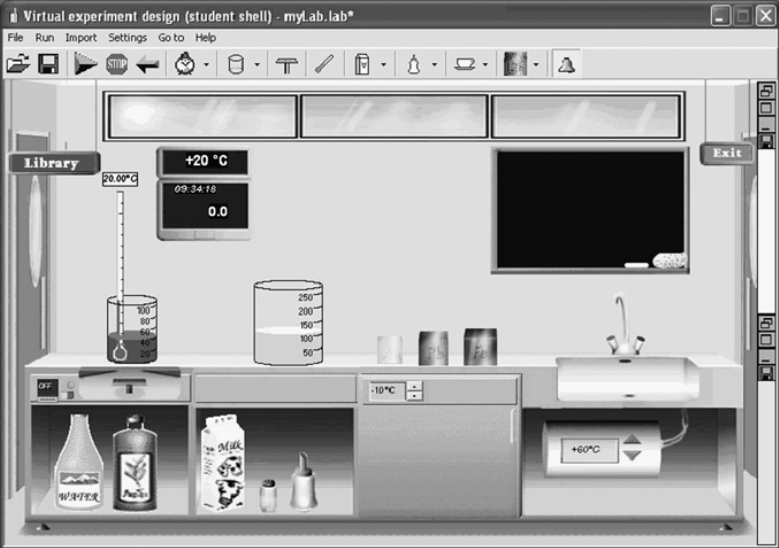
\includegraphics[width=0.90\linewidth]{chapters/works/zacharia2011.png}
	\caption{ThermoLab. Fonte:~\cite{zacharia:2011}}
	\label{fig:zacharia_thermolab}
\end{figure}

Foram realizadas quatro sessões experimentais com pré e pós-testes, onde cada teste continha 4 questões abertas e, um teste final com 8 questões abertas. Além disso, segundo os autores, não haviam itens idênticos entre o teste final e o resto dos testes e, para pontuação, foram consideradas se as respostas e as explicações das mesmas estavam certas ou erradas, onde uma resposta correta valia um ponto, e cada explicação correta valia meio ponto (uma questão poderia ter mais de uma explicação).

Com relação aos resultados, o estudo concluiu que, de modo geral, o uso de manipulativos pode contribuir tanto ou mais do que o ensino tradicional para o entendimento dos conceitos de calor e temperatura. Além disso, embora não tenham sido encontrados indícios de que o uso de manipulativos físicos é pré-requisito para o aprendizado de física, os achados corroboram que a manipulação é importante, seja ela física ou virtual. Outra descoberta diz respeito a combinação entre MF e MV, onde não foram encontradas diferenças entre iniciar com uma abordagem e prosseguir com outra ou trabalhar inteiramente com apenas uma delas.

Por fim, embora o trabalho de~\cite{zacharia:2011} tenha proposto a comparação entre o uso de objetos de aprendizagem físicos e virtuais, em nenhum dos casos há coleta de dados de interação dos estudantes com o material didático. Além disso, a experimentação envolvendo objetos físicos e virtuais mantém os dois tipos em separado, isto é, apenas físico e apenas virtual, adicionando apenas a opção metodológica de um ou outro e o seu uso consecutivo. Entretanto, um ganho importante é a evidência de que o uso de manipulativos físicos ou virtuais melhora a aprendizagem dos estudantes.

\textbf{Aprendizado de Eletrônica}\\
\cite{Salehi:2014} apresentam um estudo de menor porte, mas similar ao estudo de~\cite{zacharia:2011}, que avalia os efeitos do uso de manipulativos físicos e virtuais no aprendizado de conceitos básicos de eletrônica, mais precisamente de circuitos elétricos em série e paralelo, de acordo com as imagens apresentadas na Figura~\ref{fig:salehi2014}.

%\begin{figure}[htb]
%	\centering
%	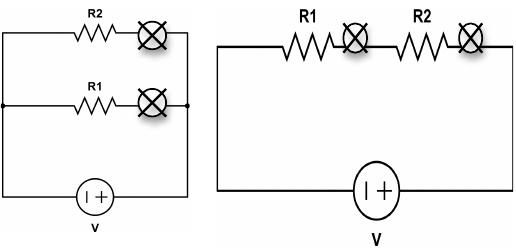
\includegraphics[width=0.6\linewidth]{imgs/salehi2014_circuito.png}
%	\caption{Esquema dos circuitos usados no estudo. Fonte:~\cite{Salehi:2014}}
%	\label{fig:salehi2014_circuitos}
%\end{figure}


\begin{figure}[htb]
	\center
	\subfigure[ref1][Manipulativo Físico]{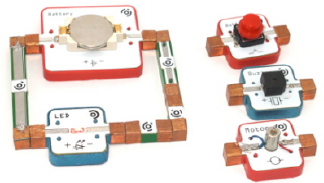
\includegraphics[width=7cm]{chapters/works/salehi-1.png}}
	\qquad
	\subfigure[ref2][Manipulativo Virtual]{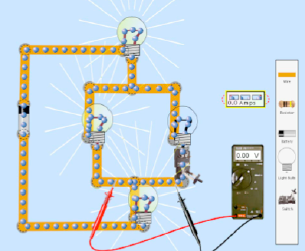
\includegraphics[width=6.4cm]{chapters/works/salehi-2.png}}
	\caption{Manipulativos usados por \cite{Salehi:2014}}
	\label{fig:salehi2014}
\end{figure}

O estudo foi feito com 32 estudantes universitários divididos em 16 pares, onde cada par trabalhou tanto com MF quanto com MV tendo que completar duas tarefas. Além disso, o experimento foi dividido em quatro blocos de acordo com a Tabela~\ref{tabela:salehi2014} e, em cada tarefa, os estudantes foram requisitados a mudar três vezes o valor de um dos resistores ($R_1$) e realizar medições de corrente e tensão dos diferentes componentes do circuito. Com esses dados, eles tiveram que elaborar teorias sobre a relação entre voltagem, corrente e resistência no circuito.
 
\begin{table}[htbp]
\caption{\textit{Design} experimental usado no estudo. Adaptado de~\cite{Salehi:2014}}
\centering
\begin{tabular}{|c|l|l|}
\hline
\textbf{Grupos} & \multicolumn{1}{c|}{\textbf{Tarefa 1}} & \multicolumn{1}{c|}{\textbf{Tarefa 2}} \\ \hline
\textbf{Bloco 1} & \begin{tabular}[c]{@{}l@{}}MV - Circuito em Série\\ 8 participantes\\ (4 pares)\end{tabular} & \begin{tabular}[c]{@{}l@{}}MF - Circuito em Paralelo\\ 8 participantes\\ (4 pares)\end{tabular} \\ \hline
\textbf{Bloco 2} & \begin{tabular}[c]{@{}l@{}}MV - Circuito em Paralelo\\ 8 participantes\\ (4 pares)\end{tabular} & \begin{tabular}[c]{@{}l@{}}MF - Circuito em Série\\ 8 participantes\\ (4 pares)\end{tabular} \\ \hline
\textbf{Bloco 3} & \begin{tabular}[c]{@{}l@{}}MF - Circuito em Série\\ 8 participantes\\ (4 pares)\end{tabular} & \begin{tabular}[c]{@{}l@{}}MV - Circuito em Paralelo\\ 8 participantes\\ (4 pares)\end{tabular} \\ \hline
\textbf{Bloco 4} & \begin{tabular}[c]{@{}l@{}}MF - Circuito em Paralelo\\ 8 participantes\\ (4 pares)\end{tabular} & \begin{tabular}[c]{@{}l@{}}MV - Circuito em Série\\ 8 participantes\\ (4 pares)\end{tabular} \\ \hline
\end{tabular}
\label{tabela:salehi2014}
\end{table}

Com relação a avaliação,~\cite{Salehi:2014} não detalham como foi calculada a pontuação ou o tipo de teste aplicado (questões abertas ou fechadas), mas afirma que para cada grupo foram executados três  testes conceituais (pré, meio e pós-teste), tendo sido calculadas as pontuações nos três testes, sendo que as pontuações dos testes do meio e pós-teste foram normalizadas a partir do pré-teste, sendo ``5'' a pontuação máxima para todos os três testes.

De modo geral, o estudo sugere que o uso de manipulativos físicos pode afetar positivamente o aprendizado e que a sequência das tarefas também pode afetar a nota final do estudante, onde os dados indicam que, para um maior ganho educacional, os manipulativos físicos deveriam ser utilizados antes dos manipulativos virtuais. Apesar disso, o artigo ainda afirma que a diferença entre iniciar com MF e prosseguir com MV ou o inverso não era estatisticamente significante, o que leva a entender que é possível inferir o mesmo que~\cite{zacharia:2011}, isto é, a ordem metodológica no uso de MF e MV não impacta substancialmente no aprendizado.

\begin{table}[htbp]
	\caption{Resumo - MF vs MV}
	\centering	
	\begin{tabular}{|l|c|c|c|c|c|c|c|c|}
		\hline
		\multicolumn{1}{|c|}{\textbf{Autor(es)}} & \textbf{MF} & \textbf{MV} & \textbf{MT} & \textbf{\begin{tabular}[c]{@{}c@{}}AE\end{tabular}} & \textbf{\begin{tabular}[c]{@{}c@{}}Coleta \\ dados\end{tabular}} & \textbf{\begin{tabular}[c]{@{}c@{}}AA\end{tabular}} & \textbf{\begin{tabular}[c]{@{}c@{}}Integração \\ com AVA\end{tabular}} & \textbf{\begin{tabular}[c]{@{}c@{}}Modelo \\ Genérico\end{tabular}} \\ \hline
		\begin{tabular}[c]{@{}l@{}}Zacharia e \\ Olympiou (2011)\end{tabular} & X & X &  & X &  &  &  &  \\ \hline
		Salehi et al. (2014) & X & X &  & X &  &  &  &  \\ \hline
	\end{tabular}
	\label{tabela:relatedsection1}
\end{table}

Assim como no trabalho de~\cite{zacharia:2011},~\cite{Salehi:2014} não coletam dados de interação dos alunos para Avaliação da Aprendizagem (AA) ou apresentam modos de calcular a aprendizagem. Além disso, embora ambos os trabalhos façam uma Avaliação Experimental (AE) e demostrem indícios de que o uso alternado de MF e MV melhorem a aprendizagem, não utilizam de manipulativos tangíveis (OT), o manipulativos utilizados não estão integrados a qualquer plataforma de aprendizagem e não apresentam um modelo genérico para a criação ou integração destes manipulativos, conforme apresentado na Tabela~\ref{tabela:relatedsection1}.

\subsection{Manipulativos Tangíveis (Físico-Digitais)}

\textbf{Melhorias nas habilidades espaciais}

\cite{ha:2018} propõem, implementam e avaliam o que chamam de ``Manipulativos Físico e Virtual ($MFV$)'' (do inglês, \textit{Virtual and Physical Manipulatives} - $VPM$), onde inserem um microcontrolador e sensores como acelerômetro, giroscópio e magnetômetro em manipulativos físicos com o objetivo de identificar as informações de orientação nos eixos x,y e z para rastrear os movimentos feitos pelos estudantes (Figura~\ref{fig:ha2018}). Além disso, cada manipulativo físico possui um correspondente ``virtual'' (Figura~\ref{fig:ha2018_VPM}) que é renderizado e movimentado de acordo com a manipulação física que o estudante executa, que o encaixa no conceito apresentado de objeto tangível.

\begin{figure}[htb]
	\centering
	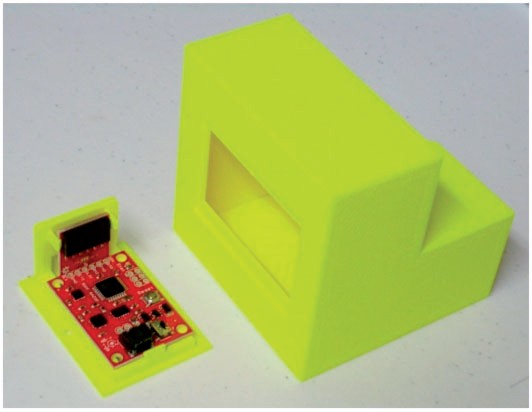
\includegraphics[width=0.7\linewidth]{chapters/works/ha2018.png}
	\caption{Manipulativo Físico com placa e sensores. Fonte:~\cite{ha:2018}}
	\label{fig:ha2018}
\end{figure}

Com o objetivo de treinar as habilidades espaciais na aula de matemática de estudantes da oitava série, especialmente no que diz respeito às habilidades de rotação mental de objetos, isto é, à capacidade de imaginar um objeto sendo rotacionado, ~\cite{ha:2018} projetaram dez tipos de $MFV$ com diferentes características geométricas de acordo com as especificações da Tabela~\ref{tab:ha2018}.

\begin{figure}[htb]
	\centering
	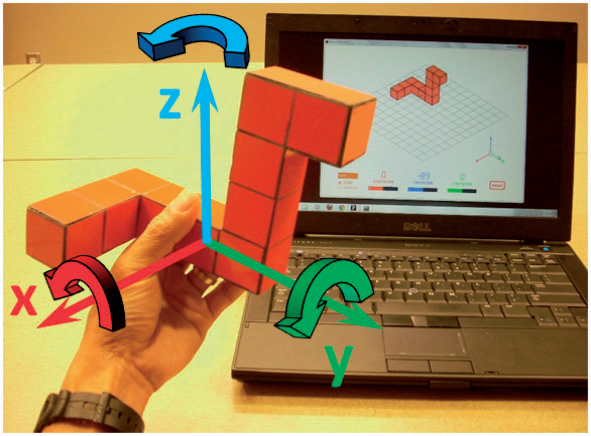
\includegraphics[width=0.7\linewidth]{chapters/works/ha2018_VPM.png}
	\caption{Manipulativo Físico e seu correspondente Virtual. Fonte:~\cite{ha:2018}}
	\label{fig:ha2018_VPM}
\end{figure}

Vale notar que os manipulativos físicos foram construídos através de impressoras 3D e os manipulativos virtuais foram projetados através do \textit{software} proprietário AutoCAD Inventor. Além disso, para avaliar os estudantes, foram realizados pré e pós-testes baseados no Teste de Visualização Espacial de Purdue (PSVT:R), que consiste em 30 questões de múltipla-escolha que ilustram um conjunto de figuras simétricas e não simétricas de objetos 3D em um formato isométrico 2D~\citep{ha:2018}.

\begin{table}[htbp]
\caption{Características Geométricas dos $MFV$ desenvolvidos por~\cite{ha:2018}}
\centering
\begin{tabular}{c|c|c|c|c|c|}
\cline{2-6}
\multicolumn{1}{l|}{} & \multicolumn{5}{c|}{\textbf{Características Geométricas}} \\ \hline
\multicolumn{1}{|c|}{\textbf{N.º}} & \textbf{\begin{tabular}[c]{@{}c@{}}Ângulo \\ Reto\end{tabular}} & \textbf{\begin{tabular}[c]{@{}c@{}}Superfícies \\ Cilíndricas\end{tabular}} & \textbf{\begin{tabular}[c]{@{}c@{}}Uma superfície \\ inclinada\end{tabular}} & \textbf{\begin{tabular}[c]{@{}c@{}}Múltiplas superfícies \\ inclinadas\end{tabular}} & \textbf{\begin{tabular}[c]{@{}c@{}}Múltiplas \\ Seções\end{tabular}} \\ \hline
\multicolumn{1}{|c|}{1} & X &  & X &  &  \\ \hline
\multicolumn{1}{|c|}{2} & X &  &  & X &  \\ \hline
\multicolumn{1}{|c|}{3} & X &  &  & X &  \\ \hline
\multicolumn{1}{|c|}{4} & X & X & X &  &  \\ \hline
\multicolumn{1}{|c|}{5} & X &  & X &  &  \\ \hline
\multicolumn{1}{|c|}{6} & X &  & X &  & X \\ \hline
\multicolumn{1}{|c|}{7} &  & X &  &  & X \\ \hline
\multicolumn{1}{|c|}{8} & X &  & X &  &  \\ \hline
\multicolumn{1}{|c|}{9} & X &  &  &  & X \\ \hline
\multicolumn{1}{|c|}{10} & X &  &  &  & X \\ \hline
\end{tabular}
\label{tab:ha2018}
\end{table}

Ao todo, sessenta e três alunos participaram das duas seções de experimento, entretanto, apenas os dados dos alunos que responderam as 30 questões foram utilizados, o que resultou em 44 alunos no pré-teste e 31 no pós-teste. A partir dos resultados de pré e pós-testes, foram calculados a pontuação de ganho e os ganhos de aprendizagem normalizados ($GAN$). As pontuações de ganho foram calculadas pela média da pontuação do pós-teste ($ps$) subtraída pela média do pré-teste ($pr$), enquanto o $GAN$ foi calculado de acordo com a Equação~\ref{equacao:hake1998}, proposta por~\cite{hake:1998}. Além disso, foram aplicados dois questionários, um de usabilidade com 21 itens baseados na Escala Likert e outro com uma questão Likert e outra aberta em que foi pedido que indicassem e justificassem a preferência por manipulativos (MF, MV ou ambos os tipos).

\begin{equation}\label{equacao:hake1998}
GAN = \frac{\% ps - \% pr}{100 - \% pr}
\end{equation}

De acordo com~\cite{ha:2018}, o uso de $MFV$ aumentou a pontuação média de todos os estudantes, onde a média no pré-teste foi 13,27(com desvio-padrão de 5,82) e a média no pós-teste foi 16,84 (com desvio-padrão de 7,58), com pontuação de ganho igual a 3,57 e ganho de aprendizagem normalizado igual a 21,3\%. O alto desvio padrão indica que as características de rotação mental é muito variável entre os estudantes analisados. Além disso, a análise estatística mostrou que a diferença entre os resultados do pré e do pós-teste é estatisticamente significativa. O mesmo aconteceu quando foram avaliados apenas os 21 estudantes que concluíram os dois testes.

Após apresentar estudos que indicam que pessoas do gênero masculino tendem a ter resultados melhores no que diz respeito a habilidades espaciais do que pessoas do gênero feminino, os dados do experimento mostram que o uso de MFV reduziu a diferença entre os gêneros de 21,5\% no pré-teste para 5,5\% no pós-teste.

Os resultados dos questionários de opinião mostram que 71,8\% dos estudantes consideram útil os MFV, 62,6\% consideram fácil de usar e, 81,3\% ficaram satisfeitos com o uso de MFV. Além do mais, a maioria dos estudantes (71,9\%) afirma preferir usar MFV do que o físico ou o virtual sozinhos porque os dois tipos de manipulativos compensam um ao outro além de alimentarem dois canais de aprendizagem (visual e tátil).

Embora, \cite{ha:2018} utilizem a expressão ``manipulativos físico e virtual'', é preciso salientar que o uso e a descrição correspondem ao que se propõe ser um manipulativo do tipo físico-digital e, portanto, objetos tangíveis de aprendizagem. Além disso, é importante notar que além de apresentar o uso de manipulativos tangíveis como uma ferramenta muito promissora para melhorar as habilidades espaciais dos estudantes, o objeto usado por \cite{ha:2018} apresentam evidências de que pode contribuir para a redução das desigualdades entre gêneros. 

Por fim, \cite{ha:2018} não oferecem elementos que garantam que o uso de manipulativos tangíveis melhorem a aprendizagem de maneira geral, não integram estes manipuláveis a uma plataforma com mecanismos de avaliação automática e/ou extraem dados de interação para análise de aprendizagem. Além disso, embora utilize questionários de múltipla-escolha, não fica claro como a pontuação dos alunos é calculada, o que permite supor que é utilizada a ``Pontuação Tradicional'' (Seção~\ref{sec:nota-tradicional}), isto é, levando em consideração unicamente se a resposta escolhida pelo aluno está certa ou errada.

\textbf{Disciplinas STEM}

\cite{Azad:2016} contextualizam seu trabalho em STEM, sigla em inglês que designa as seguintes áreas do conhecimento: Ciências, Tecnologia, Engenharia e Matemática, e em Internet das Coisas (IoT) apontando a importância do uso de sistemas ciberfísicos em uma abordagem educacional que seja interdisciplinar.

\begin{figure}[htb]
	\centering
	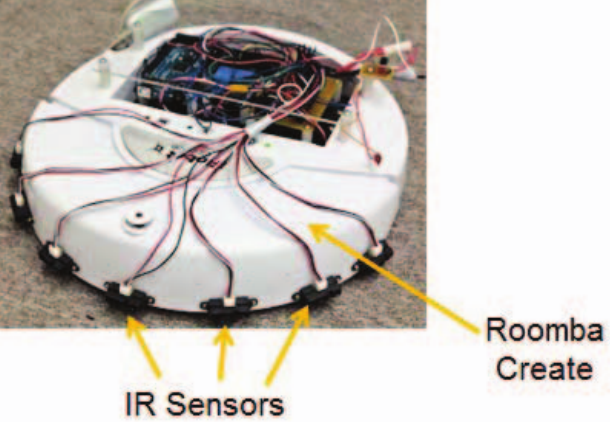
\includegraphics[width=0.6\linewidth]{chapters/works/azad2016.png}
	\captionsetup{justification=centering}
	\caption{RoCr com Arduíno e sensores infravermelho integrados. \\Fonte:~\cite{Azad:2016}}
	\label{fig:azad2016}
\end{figure}

Após uma introdução acerca da estrutura de sistemas ciberfísicos,~\cite{Azad:2016} apresentam três casos de estudo: (i) Casa Inteligente, com uso de Arduíno e sensores de luz e temperatura para controle automático de portas e de um equipamento de ventilação para ajuste da temperatura interna da casa, além de monitoramento remoto pelo usuário; (ii) \textit{Roomba Create} (RoCr), desenvolvido pela empresa \textit{iRobot}, que permite programar o comportamento do robô e que foi modificado para ser controlado remotamente pelo usuário ou funcionar de modo automático, tendo sido adicionados sensores de infravermelho e um Arduíno Mega (Figura~\ref{fig:azad2016}); e, (iii) sistemas embarcados de programação remota, que consiste em uma placa Arduíno com \textit{display} LCD, LEDs, motor de passos e um \textit{display} 7 segmentos com acesso remoto, conforme mostrado na Figura~\ref{fig:azad2016_remote}.

\begin{figure}[htb]
\center
\subfigure[ref1][Imagem da parte física]{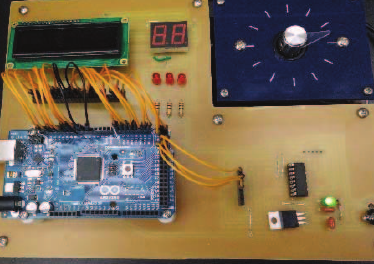
\includegraphics[width=7cm]{chapters/works/azad2016_remote1.png}}
\qquad
\subfigure[ref2][Imagem da GUI ]{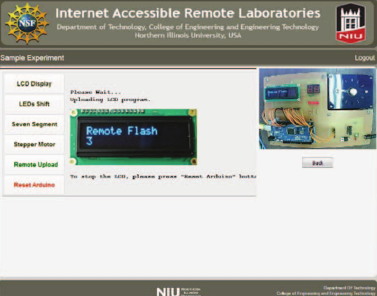
\includegraphics[width=6.4cm]{chapters/works/azad2016_remote2.png}}
\captionsetup{justification=centering}
\caption{Sistemas Embarcados de Programação Remota. \\Fonte:~\cite{Azad:2016}}
\label{fig:azad2016_remote}
\end{figure}

Com exceção do último caso, que utiliza Python no desenvolvimento, as propostas de~\cite{Azad:2016} utilizam a plataforma LabVIEW para implementação dos sistemas. Além disso, embora o trabalho seja contextualizado em STEM, os casos de uso apresentados não estão necessariamente aplicados no contexto educacional, além de não apontar elementos de coleta de dados, de integração a qualquer plataforma educacional ou de avaliação da aprendizagem.

\subsection{Modelagem Bifocal}

\cite{Blikstein:2012} e \cite{Blikstein2016} apresentam estudos que utilizam um \textit{framework} chamado Modelagem Bifocal (MB), onde manipulativos físicos e virtuais são justapostos. Segundo~\cite{Blikstein:2012}, no modelo bifocal, os estudantes constroem tanto um modelo físico, com sensores de um dado fenômeno científico, quanto um modelo virtual do mesmo fenômeno, conectando ambos em tempo real através de uma interface especial de \textit{hardware}, com o objetivo de compará-los.

De acordo com~\cite{Blikstein:2012}, a construção de um modelo bifocal implica que três tarefas principais sejam executadas pelos estudantes: (i) projetar um modelo físico para estudar o fenômeno científico usando sensores eletrônicos e a placa de baixo custo Gogo~\citep{sipitakiat:2003}; (ii) projetar um modelo virtual de computador do mesmo fenômeno usando um \textit{software} de modelagem, onde, normalmente, é usado o NetLogo, que é um ambiente de código-aberto e gratuito para modelagem baseada em agentes); e, (iii) conectar e executar ambos os modelos para compará-los e depurá-los.

\begin{figure}[htb]
	\centering
	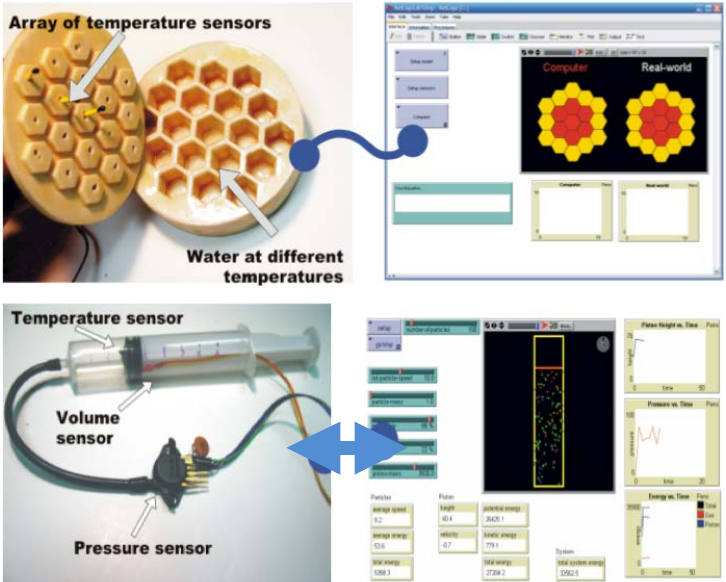
\includegraphics[width=0.8\linewidth]{chapters/works/blikstein2012.png}
	\captionsetup{justification=centering}
	\caption{Exemplos de Modelos Bifocais: transferência de calor e leis dos gases. Fonte:~\cite{Blikstein:2012}}
	\label{fig:blikstein2012}
\end{figure}

Desse modo,~\cite{Blikstein:2012} apresentam um prova de conceito com quatro estudos-piloto aplicando a MB na aprendizagem de fenômenos científicos em biologia, química e física em estudantes de ensino médio nos Estados Unidos. Os estudos consistiram em investigar e analisar padrão de crescimento de bactérias, leis de Newton a partir do tempo de uma bola descendo uma rampa, relação entre volume e pressão em um sistema fechado e difusão líquida. A Figura~\ref{fig:blikstein2012} apresenta dois exemplos de modelos bifocais propostos em~\cite{Blikstein:2012}, onde a esquerda podemos observar os manipulativos físicos e a direita os virtuais.

Além disso,~\cite{Blikstein:2012} dividiram as modelagens física e virtual em sequências de atividades menores que consistiram em: (i) pesquisa inicial para busca de fundamentos; (ii) projeto dos modelos com seleção de variáveis a ser observadas e construção de hipóteses a ser testadas; (iii) construção dos modelos físicos e virtuais para estudo do fenômeno; e, (iv) interação dos estudantes com os próprios modelos para observação, coleta de dados ou mudança de parâmetros. 

Com relação aos resultados, \cite{Blikstein:2012} apenas foca em como os estudantes resolveram as diferenças entre os modelos reais e virtuais, não apresentando estratégias de avaliação da aprendizagem ou se a abordagem de modelagem bifocal fez alguma diferença na aprendizagem das disciplinas propostas no estudo. Além disso, outra característica tanto de~\cite{Blikstein:2012} quanto de~\cite{Blikstein2016} é a metodologia baseada no trabalho de~\cite{Papert:1980} e~\cite{Papert:1994}.

\begin{table}[htbp]
	\caption{Resumo - Manipulativos Tangíveis}
	\centering
	\begin{tabular}{|l|c|c|c|c|c|c|c|c|}
		\hline
		\multicolumn{1}{|c|}{\textbf{Autor(es)}} & \textbf{MF} & \textbf{MV} & \textbf{MT} & \textbf{AE} & \textbf{\begin{tabular}[c]{@{}c@{}}Coleta\\ dados\end{tabular}} & \textbf{AA} & \textbf{\begin{tabular}[c]{@{}c@{}}Integração \\ com AVA\end{tabular}} & \textbf{\begin{tabular}[c]{@{}c@{}}Modelo\\ Genérico\end{tabular}} \\ \hline
		Ha Fang (2018) &  &  & X & X &  &  &  &  \\ \hline
		\begin{tabular}[c]{@{}l@{}}Azad e \\ Hashemian (2016)\end{tabular} &  &  & X &  &  &  &  &  \\ \hline
		\begin{tabular}[c]{@{}l@{}}Blikstein et \\ al. (2012) e (2016)\end{tabular} & X & X & X &  & X &  &  &  \\ \hline
	\end{tabular}
	\label{tabela:relatedsection2}
\end{table}

Por fim, a Tabela~\ref{tabela:relatedsection2} apresenta um resumo do apresentado nesta seção, de modo que é possível notar que, embora os trabalhos abordem a construção e o uso de manipulativos tangíveis, nenhum apresenta elementos para Avaliação da Aprendizagem (AA), Integração com Ambientes Virtuais de Aprendizagem (AVA) ou um modelo genérico para construção de objetos tangíveis compatíveis com alguma plataforma. Além disso, apenas uma abordagem proporciona coleta de dados, sendo que tal coleta não está relacionada a avaliação ou acompanhamento da aprendizagem através de dados provenientes da interação com os objetos de aprendizagem.

\subsection{Sistemas Físico-Virtuais de Aprendizagem no Brasil}

Nossa busca nas bases de dados da ``Comissão Especial de Informática na Educação'' (CEIE) da Sociedade Brasileira de Computação (SBC), que é a principal base brasileira de publicações na área de informática na educação, retornou apenas duas publicações evidentemente relacionadas a construção de ambientes baseados a sistemas ciberfísicos no contexto educacional no Brasil e que utilizam o termo ``físico-virtual'' ao invés de ``tangível''. Em contrapartida, uma grande quantidade de trabalhos recentes alinha-se ao desenvolvimento de ambientes tangíveis de aprendizagem.

\textbf{Plataforma Toogle}

\cite{Santos:2014} apresentam uma proposta embrionária de um ambiente físico-virtual de aprendizagem e uma plataforma para implementação de sistemas físico-virtuais, cuja arquitetura (Figura~\ref{fig:santos2014plataforma}) contém quatro módulos: (i) \textbf{\textit{Middleware} e Componentes:} proporciona comunicação entre as entidades físicas e virtuais do ambiente, sendo composto pelo \textit{framework} ROS (\textit{Robot Operating System}) que, por meio de ferramentas e bibliotecas próprias, fornece uma abstração de \textit{hardware}, \textit{drivers} para diversos dispositivos e um sistema de troca de mensagens; (ii) \textbf{Toogle Editor:} módulo que utiliza a ferramenta \textit{Blender} para adicionar, remover e editar componentes físico-virtuais, além dos objetivos do ambiente; (iii) \textbf{Inteligência de Ambiente:} fornece um conjunto ordenado de recursos para conduzir o ambiente ao alcance dos objetivos estabelecidos; e, (iv) \textbf{Toogle Navegador:} possibilita a interação dos usuários com o ambiente, provendo por exemplo, informações sonoras, estereoscópicas, táteis, dentre outras, além de um \textit{plugin} para Web. 
Além disso, o trabalho publicado por~\cite{Santos:2014} é derivado da tese de doutorado do mesmo autor principal, isto é~\cite{santos:2014ambientes}, igualmente defendida em 2014. 

\begin{figure}[htb]
	\centering
	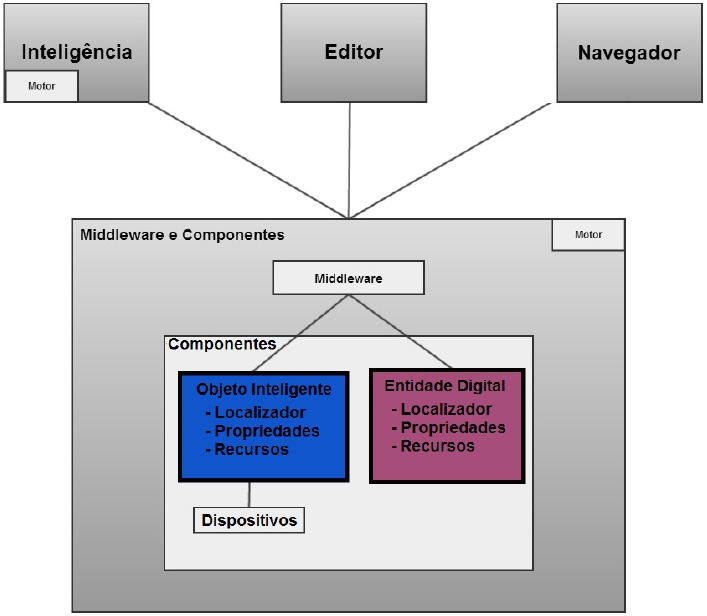
\includegraphics[width=0.8\linewidth]{chapters/works/santos2014_arquitetura.png}
	\caption{Arquitetura da Plataforma Toogle. Fonte:~\cite{Santos:2014}}
	\label{fig:santos2014plataforma}
\end{figure}

Após apresentar a plataforma Toogle e baseando-se no trabalho de~\cite{xu:2005}, que apresenta um modelo conceitual para um ambiente virtual de aprendizagem construtivista, ~\cite{Santos:2014} e~\cite{santos:2014ambientes} propõem um modelo conceitual para ambientes físico-virtuais de aprendizagem (Figura~\ref{fig:santos2014modelo}), o qual está relacionado com a plataforma apresentada. Tal modelo contém os sete elementos a seguir: (i) \textbf{aluno e contexto:} ``alunos'' são identificados como atores que interagem com o ambiente com o objetivo de aprender, enquanto o ``contexto'' pode ajudar nos momentos de aprendizagem, por exemplo, estabelecendo novos conteúdos; (ii) \textbf{professores: } elaboram os currículos, determinam os objetivos de aprendizagem e mediam as adaptações (oportunismo) das situações de aprendizagem; (iii) \textbf{situação: } formaliza o contexto da situações de aprendizagem usando a abordagem de solução de problemas \textit{STRIPS}, proposta por~\cite{fikes:1971}, além de oferecer novas oportunidades para o ensino; (iv) \textbf{oportunismo: }sugerir situações de aprendizagem (com elementos físicos e virtuais) baseando-se nas interações prévias ou atuais dos estudantes; (v) \textbf{interação: }proporciona espaços de interação em que há a mistura de elementos físicos e virtuais; (vi) \textbf{objetivos de aprendizagem: } indicados pelo professor, são o enfoque das atividades; (vii) \textbf{currículo:} armazena as informações do currículo, além de possibilitar que o professor desenvolva objetos de aprendizagem que sejam físico-virtuais.

\begin{figure}[htb]
	\centering
	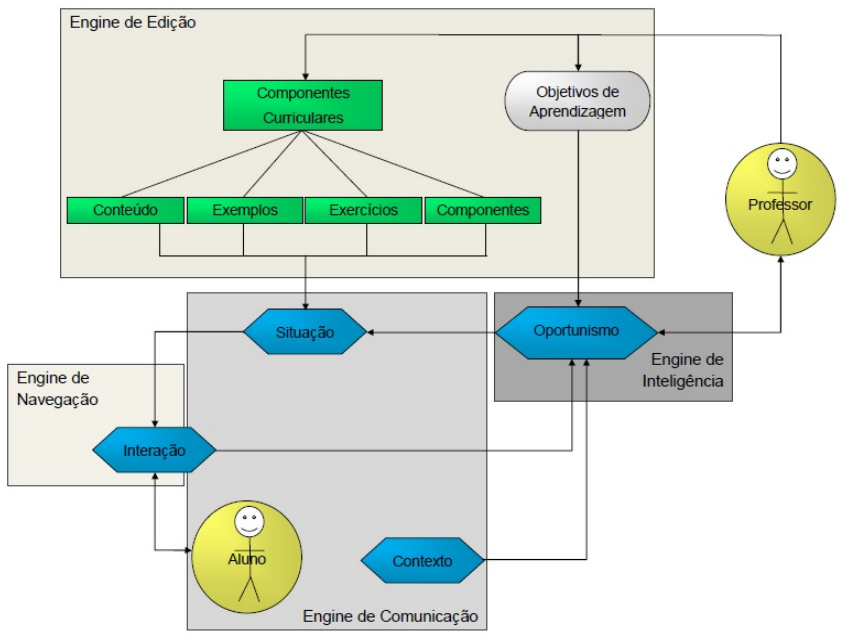
\includegraphics[width=0.9\linewidth]{chapters/works/santos2014_modelo_v2.png}
	\captionsetup{justification=centering}
	\caption{Modelo Conceitual de um Ambiente Físico-Virtual de Aprendizagem proposto por~\cite{santos:2014ambientes}}
	\label{fig:santos2014modelo}
\end{figure}

O estudo de caso de~\cite{Santos:2014} foi a criação de uma aula com os seguintes componentes: sala de aula, aluno, professor, apostila 1, apostila 2 e \textit{smartphone}. Desse modo, foi introduzido um modelo em 3D de um prédio com várias salas de aula às quais foram associadas coordenadas de GPS que serviriam de gatilho para a visualização de apostilas em PDF, sendo a visualização das mesmas o objetivo de aprendizagem definido pelo professor. Além disso, o componente \textit{smartphone} estaria associado a um componente ``prevê\_posição'' para que as posições do aluno fossem coletadas e, então, se verificasse se a posição atual coincide com a posição do objetivo de aprendizagem.

A comunicação entre os diversos módulos da plataforma acontece através de arquivos XML que, por último, são enviados ao módulo de ``inteligência do ambiente'' que planeja a execução dos recursos. O artigo não detalha o modo como esse planejamento acontece, embora mencione que a execução das ações acontece mediante verificação das propriedades dos recursos, por exemplo, enquanto a apostila não tiver sido visualizada, o sistema pode enviá-la assim que determinado estudante atingir a localização geográfica associada a ela.

\cite{Santos:2014} concentra-se somente em definir uma arquitetura geral de como deveria ser um ambiente físico-virtual de aprendizagem e em implementar um exemplo dessa arquitetura, sem desenvolver/aplicar ferramentas/estratégias de gerência ou avaliação da aprendizagem e sem explorar dados relacionados a interação dos alunos com o material didático. Além disso, a plataforma e o modelo apresentados cobrem efetivamente apenas quatro dos oito requisitos requisitos de um ambiente físico-virtual de aprendizagem definidos por~\cite{santos:2014ambientes}.

\textbf{Leitura colaborativa em ambiente físico-virtual}

O trabalho de~\cite{imamura:2018} segue uma linha de leitura colaborativa que toma por base o construtivismo e o enativismo, onde, de acordo com os autores, no primeiro caso, o conhecimento é tido como algo a ser construído a partir das relações físicas e sociais estabelecidas pelos indivíduos e, no segundo, o conhecimento está relacionado a uma descoberta pela ação, a uma sensorialidade ou a uma experimentação do mundo físico~\citep{imamura:2018}. 

Assim, a pesquisa de~\cite{imamura:2018} utiliza realidade aumentada para viabilizar a implementação de um sistema socioenativo de Leitura Colaborativa Físico-Virtual (LCFV) que leva em consideração a exploração física do espaço por meio de uma aplicação para \textit{smartphones}, conforme mostrado na Figura~\ref{fig:imamura2018}.

O primeiro protótipo do projeto utilizou \textit{QR Codes} em cada objeto físico para dar acesso a sua representação e conteúdo virtuais e para o cenário de leitura foi criada uma narrativa baseada em um desafio onde o objetivo dos participantes era descobrir o que aconteceu usando informações do ambiente físico-virtual. Embora o primeiro experimento tenha sido feito com quatro estudantes de pós-graduação, o desafio foi proposto para ser aplicado a crianças de 10 anos que visitassem o Museu Exploratório de Ciências da Unicamp.

\begin{figure}[htb]
	\centering
	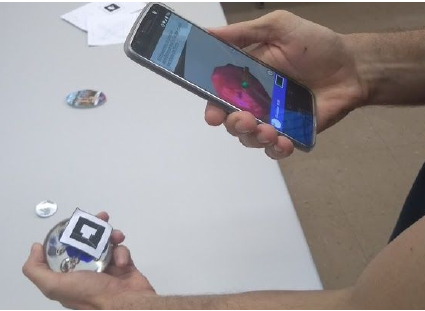
\includegraphics[width=0.6\linewidth]{chapters/works/imamura2018.png}
	\captionsetup{justification=centering}
	\caption{Exemplo de exploração do cenário físico usando \textit{smartphone}. Fonte:~\cite{imamura:2018}}
	\label{fig:imamura2018}
\end{figure}

\cite{imamura:2018} indicam que o primeiro protótipo para LCFV foi implementado de modo que cada grupo tivesse 4 leitores e um moderador que conhece o funcionamento da história, tendo sido utilizados 14 objetos físicos com \textit{QR Code} e 5 objetos sem interações virtuais diretas. Além disso, cada leitor recebe um papel diferente (cientista, programador, atleta e professor), onde cada um terá acesso a diferentes informações do objeto físico durante dois minutos. Assim, há um rodízio que faz com que, enquanto um membro do grupo ``explora'' o cenário, os outros levantam questionamentos e hipóteses que ajudem a compor a narrativa (Figura~\ref{fig:imamura2018_LCFV}).

\begin{figure}[htb]
	\centering
	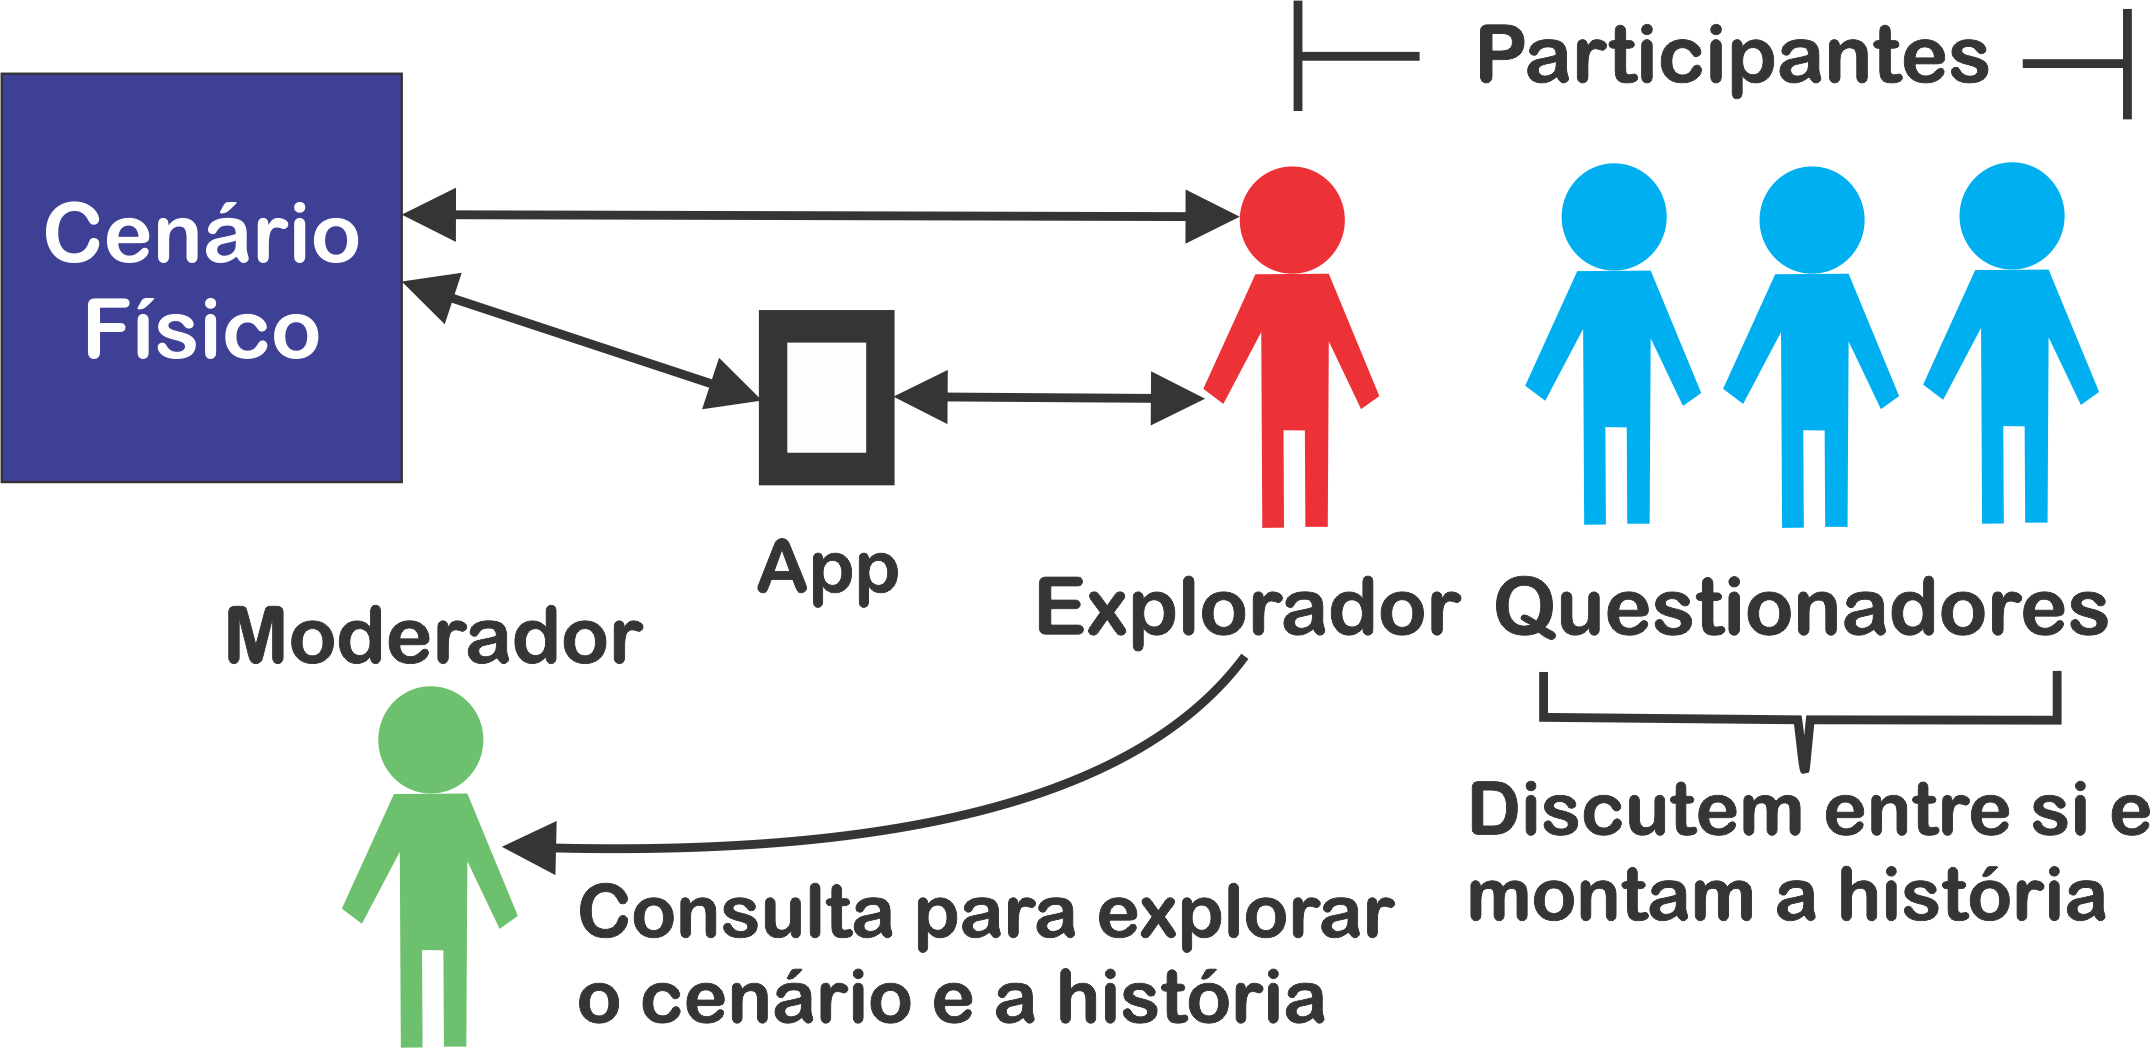
\includegraphics[width=0.7\linewidth]{chapters/works/imamura2018_LCFV.png}
	\captionsetup{justification=centering}	
	\caption{Configuração da LCFV para o primeiro experimento. \\Fonte:~\cite{imamura:2018}}
	\label{fig:imamura2018_LCFV}
\end{figure}

Segundo~\cite{imamura:2018}, a leitura colaborativa deve resultar em ``um texto estruturado por imagens, colagens, diagramas e falas dos participantes''. Além disso, os participantes também tem disponíveis objetos que ajudem a organizar as informações, tais como materiais de escrita, \textit{post-it} e um espaço para colocar as perguntas envolvendo a história, reflexões resultantes da experiência, conexões feitas entre o que foi explorado e o mundo exterior.

Após a atividade, foi feita uma avaliação utilizando um questionário AttrakDiff que, de acordo com~\cite{imamura:2018}, usa uma escala semântica de -3 a 3 para avaliar aspectos da experiência do usuário tais como atratividade, estímulo e qualidade pragmática e hedônica. Assim, de acordo com essa avaliação, a experiência dos usuários foi expressa através de palavras com 100\% de concordância dos participantes (`agradável',`convidativo', `criativo', `cativante' e `motivadora'), com concordância acima de 80\% (`prática', `integradora', `boa', `inovadora', `desafiadora', `nova', `profissional', `imprevisível' e `apresentável'). Além disso, houve menos concordância a respeito se a experiência foi `confusa' ou `claramente estruturada'.

Embora proponha algo muito inovador, não somente pela inserção de sistemas ciberfísicos, mas também pela proposta de leitura colaborativa com uma abordagem socioenativa, o trabalho de~\cite{imamura:2018}
não prevê um modo de avaliar automaticamente a aprendizagem dos estudantes (especialmente por que o cenário demanda algum nível de imprevisibilidade) e não utiliza os elementos tangíveis em associação a uma plataforma educacional mais ampla.

\textbf{Objetos Tangíveis no Ensino de Matemática}

\cite{lima:2016} apresentam uma proposta de design colaborativo de objetos tangíveis para crianças e uma versão tangível do Tangram que fornece \textit{feedback} automático aos estudantes e professores com relação a posição das peças (se foram colocadas corretamente ou não). De acordo com os autores, o jogo Tangram possibilita o aprendizado de conceitos geométricos de frações, lados, ângulos, formatos semelhantes, perímetro e área de figuras planas, semelhanças de triângulos, ângulos e polígonos congruentes.

\begin{figure}[htb]
	\centering
	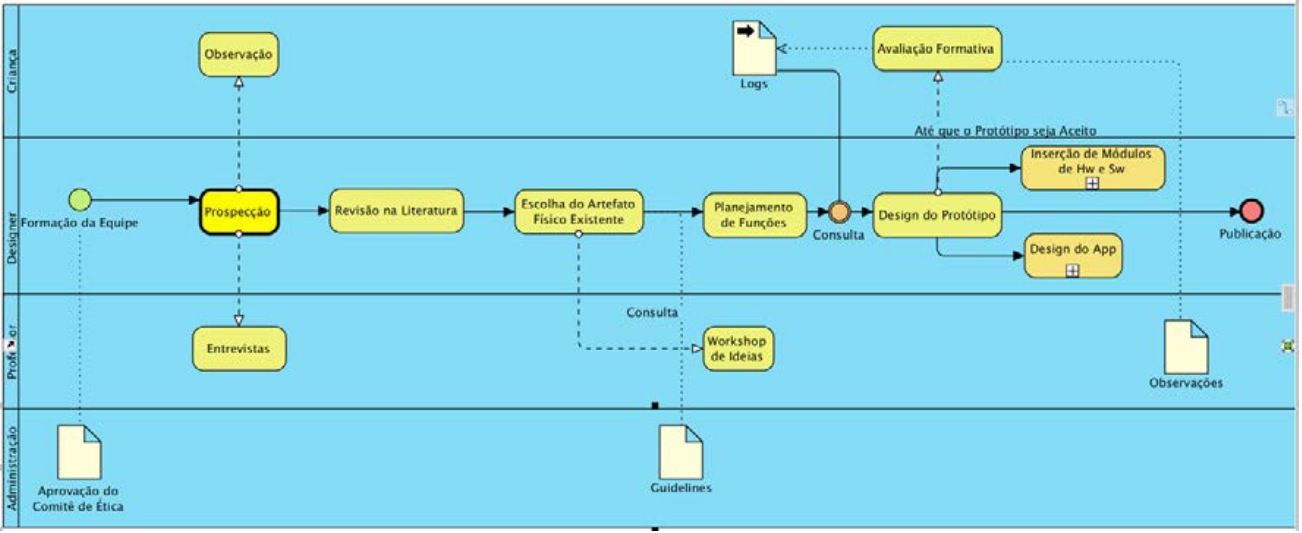
\includegraphics[width=1\linewidth]{chapters/works/lima2016.png}
	\captionsetup{justification=centering}	
	\caption{Processo de Design em Artefatos Tangíveis para Crianças. \\Fonte:~\cite{lima:2016}}
	\label{fig:lima2016}
\end{figure}

Como parte da metodologia utilizada, uma abordagem baseada em Design Participativo foi adaptada de modo que o objeto tangível fosse gerado a partir da observação e colaboração de crianças que utilizariam o jogo, além disso é apresentada uma descrição do modelo de processo utilizando diagrama BPMN (Figura~\ref{fig:lima2016}).

\begin{figure}[htb]
	\center
	\subfigure[ref1][Peça com sensores e Arduíno embutidos ]{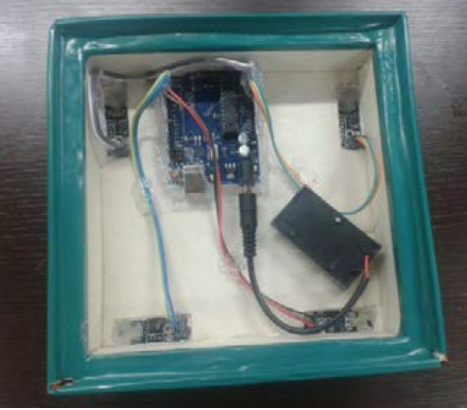
\includegraphics[width=7cm]{chapters/works/lima2016-2.png}}
	\qquad
	\subfigure[ref2][Peças do Tangram instrumentadas com sensores ]{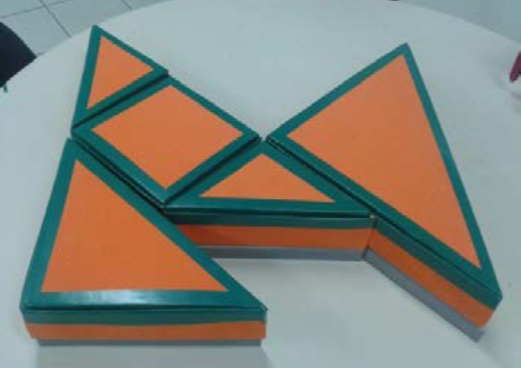
\includegraphics[width=6.4cm]{chapters/works/lima2016-3.png}}
	\captionsetup{justification=centering}
	\caption{Protótipo do Tangram Tangível}
	\label{fig:lima2016_prototipo}
\end{figure}

Foram elaborados dois protótipos funcionais, onde o primeiro protótipo foi apenas uma prévia para o segundo, de modo que os  materiais utilizados na construção das sete peças do Tangram no protótipo final (Figura~\ref{fig:lima2016_prototipo}) foram: ``Arduíno Uno, Sensor \textit{Hall}, \textit{Shield Bluetooth}, \textit{Jumper wires}, Cabo USB, LED, Tecido inteligente, Cartolina, Emborrachado, Papelão Branco, Régua, Lápis, Pincel e Fitas''. 
Como parte da proposta do jogo, foi implementado um aplicativo Android (Figura~\ref{fig:lima2016_app}) com imagens que deveriam ser selecionadas pelos estudantes e replicadas utilizando o objeto tangível.

\begin{figure}[htb]
	\centering
	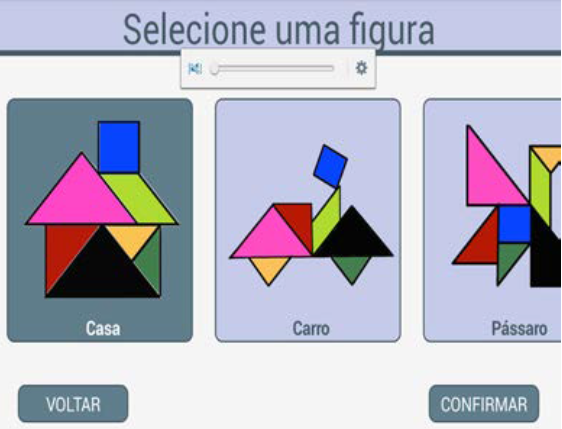
\includegraphics[width=0.6\linewidth]{chapters/works/lima2016-4.png}
	\caption{Tela do App para o Tangram Tangível. \\Fonte:~\cite{lima:2016}}
	\label{fig:lima2016_app}
\end{figure}

Por fim, é importante salientar que, embora o trabalho comente sobre o fornecimento de um \textit{feedback} para estudantes e professores e sobre uma avaliação formativa ter sido realizada, não são apresentados mais detalhes além de que essa avaliação fez parte do processo de construção dos protótipos. Além disso, o trabalho não prevê um método de avaliação da aprendizagem usando dados coletados pelo objeto tangível, bem como o protótipo não está integrado a qualquer ambiente de aprendizagem mais abrangente.

\textbf{Ambiente Virtual Tangível no Ensino de Ciências}

\begin{figure}[htb]
	\centering
	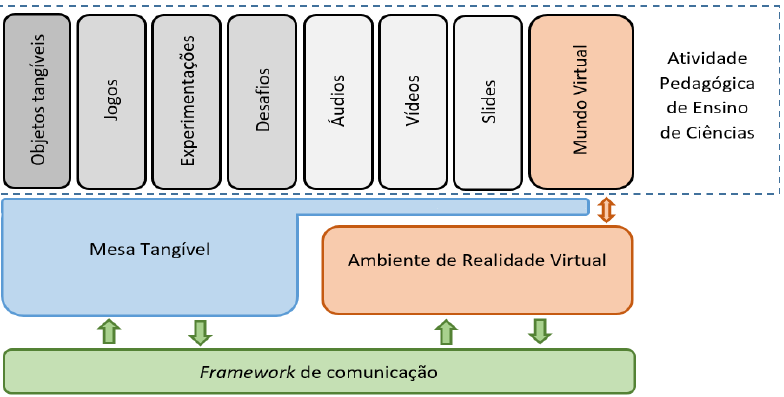
\includegraphics[width=0.8\linewidth]{chapters/works/gluz2018.png}
	\captionsetup{justification=centering}
	\caption{Integração da MT e RV numa atividade pedagógica. \\Fonte:~\cite{gluz:2018}}
	\label{fig:gluz2018-framework}
\end{figure}

\cite{gluz:2018} apresentam uma proposta de ambiente de aprendizagem que utiliza objetos tangíveis e realidade virtual 3D, que denominam de ``Ambiente de ensino Virtual Tangível (AVT)'', cujo objetivo é auxiliar no ensino de Ciências numa perspectiva inclusiva, com estudantes que tem déficit de comunicação.

Como objeto tangível é utilizada uma Mesa Tangível (MT), que provê uma superfície onde os estudantes podem manipular os objetos de modo que essa manipulação física seja comunicada a um ambiente de Realidade Virtual (RV) 3D através de um \textit{framework} especialmente construído para isso. A Figura~\ref{fig:gluz2018-framework} apresenta como as partes desse ambiente se comunicam.

De acordo com \cite{gluz:2018}, a construção da MT contou com os seguintes materiais: estrutura de madeira, superfície de acrílico e vinil translúcido, LEDs de infravermelho, projetor, câmera de infravermelho e um computador. O software da MT é composto de um editor, um player e uma biblioteca de protocolos de comunicação, tendo sido desenvolvido utilizando tecnologias web como HTML5 e JavaScript. Além disso, a comunicação com a RV é feita através de \textit{web services}.

\begin{figure}[htb]
	\centering
	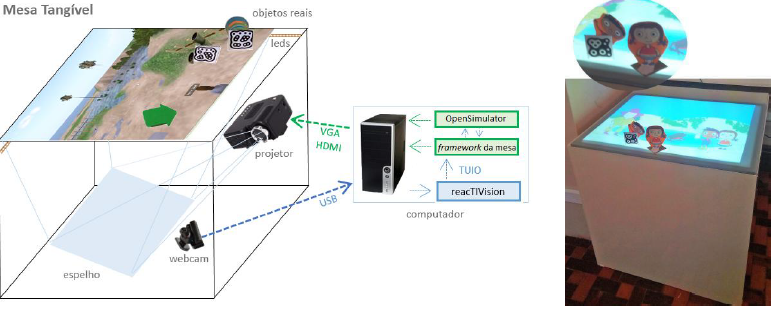
\includegraphics[width=0.9\linewidth]{chapters/works/gluz2018-mesa.png}
	\caption{Estrutura e componentes da mesa tangível. \\Fonte:~\cite{gluz:2018}}
	\label{fig:gluz2018-mesa}
\end{figure}

A Figura~\ref{fig:gluz2018-mesa} apresenta o esquema dos componentes da mesa tangível e uma imagem da mesa real construída, onde se pode observar a superfície tangível através da qual os estudantes interagem com o ambiente virtual utilizando objetos físicos. 

No contexto da proposta apresentada por \cite{gluz:2018}, o AVT apresenta uma história educativa ambientada no Parque Estadual de Itapeva (RS) contendo quatro personagens com diferentes funções dentro da história e que interagem com os estudantes como um agente pedagógico inteligente cujo objetivo é explicar, guiar, interagir e lançar desafios aos estudantes.

Ademais, o trabalho apresentado é centrado na descrição do desenvolvimento do ambiente virtual e da prova de conceito, inclusive apresentando a proposta de roteiro da história implementada, de modo que os próprios autores comentam que o próximo seria a realização de experimentos empíricos em sala de aula. Assim, o ambiente virtual tangível, sendo uma proposta ambiente educacional, possibilita o uso de diferentes objetos de aprendizagem (objetos tangíveis, jogos, desafios, áudios, vídeos, slides,...), mas, não pressupõe alguma abordagem de avaliação da aprendizagem ou coleta de dados de interação dos estudantes com a mesa tangível.


Por fim, a Tabela~\ref{tabela:relatedsection_br} apresenta um resumo dos trabalhos desta seção, de modo a melhor comparar as suas características. Assim, nenhum dos trabalhos apresenta isoladamente um objeto físico ou virtual, mas, objetos que podem ser considerados tangíveis, uma vez que tais objetos contém elementos físicos e virtuais que, de algum modo, estão integrados entre si. Apenas dois trabalhos fazem uma Avaliação Experimental (AE) \citep{imamura:2018,lima:2016}, dois trabalhos tem algum tipo de integração com um ambiente de aprendizagem \citep{santos:2014ambientes, gluz:2018}, embora \cite{santos:2014ambientes} apresente um modelo e uma instância de um ambiente `físico-virtual' que provê objetos tradicionais e, outros dois trabalhos \citep{santos:2014ambientes,lima:2016} apresentam modelos genéricos relacionados a objetos físico-virtuais (tangíveis). É importante notar que nenhum dos trabalhos apresenta coleta de dados e nem avaliação da aprendizagem, inclusive através de dados provenientes destas coletas.

\begin{table}[htbp]
	\caption{Resumo - Sistemas Físico-Virtuais no Brasil}
	\centering
	\begin{tabular}{|l|c|c|c|c|c|c|c|c|}
		\hline
		\multicolumn{1}{|c|}{\textbf{Autor(es)}} &
		\textbf{MF} &
		\textbf{MV} &
		\textbf{MT} &
		\textbf{AE} &
		\textbf{\begin{tabular}[c]{@{}c@{}}Coleta\\ dados\end{tabular}} &
		\textbf{AA} &
		\textbf{\begin{tabular}[c]{@{}c@{}}Integração \\ com AVA\end{tabular}} &
		\textbf{\begin{tabular}[c]{@{}c@{}}Modelo\\ Genérico\end{tabular}} \\ \hline
		Santos et al. (2014)                                                    &  &  &   &   &  &  & X & X \\ \hline
		\begin{tabular}[c]{@{}l@{}}Imamura e \\ Baranauskas (2018)\end{tabular} &  &  & X & X &  &  &   &   \\ \hline
		Lima et al. (2016)                                                      &  &  & X & X &  &  &   & X \\ \hline
		Gluz et al. (2018)                                                      &  &  & X &   &  &  & X &   \\ \hline
	\end{tabular}
	\label{tabela:relatedsection_br}
\end{table}

% \section{Ambientes de Aprendizagem} 
% \label{section:LearninAmbients}

% \cite{Garcia:2010} afirma que há dois tipos de aprendizado: o formal, que ocorre dentro da sala de aula, e o informal, que acontece fora dela. O primeiro tipo é mais comum na educação escolar tradicional, entretanto, o segundo tipo inclui todos os lugares que não sejam, à primeira vista, um ambiente de sala de aula em si. Nessa perspectiva, a casa do estudante, um museu, um parque, ou qualquer outro local pode ser considerado ambiente de aprendizagem, visto que está passível de ocorrer nele uma situação de aprendizado informal. Considerando esses fatores, classificaremos os ambientes de sala de aula inteligente em dois tipos:

% \begin{enumerate}
% 	\item \textbf{Ambiente interno:} são aqueles desenvolvidos num contexto de salas de aula formal. Trabalhos relacionados ao ensino à distância, ao uso de dispositivos móveis, sensores ou computadores vestíveis que necessitem da presença dos estudantes e do professor simultaneamente e que simule uma sala de aula formal também estão contidos nesta classificação. 
	
% 	\item \textbf{Ambiente externo:} contextos educacionais ao ar livre o que implica em ambientes mais abertos como museus, zoológicos, parques, ou até mesmo a casa do estudante. Trabalhos relacionados ao ensino à distância, ao uso de dispositivos móveis, sensores ou computadores vestíveis que permitam mobilidade e liberdade dos estudantes em relação ao conteúdo e tempo de estudo também se encaixam nessa classificação.
% \end{enumerate}

% % -----------------------------------------------------------------
% => Ambiente Interno
% -----------------------------------------------------------------

\subsection{Ambiente Interno de Aprendizagem}
\label{section:wIndoorClassroom}

%Abordagens de construção de ambientes ou componentes de sala de aula presencial tem sido objeto de estudo de alguns trabalhos, em geral, esses trabalhos enfocam o uso de RFID (\textit{Radio-Frequency IDentification}), câmeras, servidores, novos tipos de mobiliário, lousas inteligentes e dispositivos móveis.

\cite{Bargaoui:2014} apresentam um \textit{Gateway} para conectar os múltiplos dispositivos utilizados numa sala de aula inteligente. Para construção da solução são utilizados RFID, servidor de dados, ferramentas de administração, lousa inteligente, \textit{Raspberry-Pi}, OSGi (\textit{Open Service Gateway Initiative}) e dispositivos inteligentes diversos. Como trabalhos futuros, é sugerida a criação de um modelo de avaliação da experiência do estudante e compará-lo com uma sala de aula clássica.

\cite{Margetis:2011} descrevem uma abordagem a partir da aplicação de Inteligência de Ambientes em sala de aula e faz um levantamento de requisitos importantes a serem levados em consideração a fim de ajudar de modo mais eficiente na melhoria da educação dos estudantes. Utiliza um \textit{framework} chamado ClassMATE (\textit{Classroom Multiplatform Augmented Technology Environment}) dentre outras ferramentas como: FAMINE (\textit{FORTH's AMI Network Environment}), PERSONAF (\textit{Personalised Pervasive Scrutable Ontological Framework}), \textit{Learning Technology Systems Architecture} (LTSA), Desk aumentado, lousa inteligente, PUPIL (um \textit{front-end educacional}) que são aplicações eletrônicas para sala de aula (Figura~\ref{fig:margetis2011}).

\begin{figure}[ht]
\centering
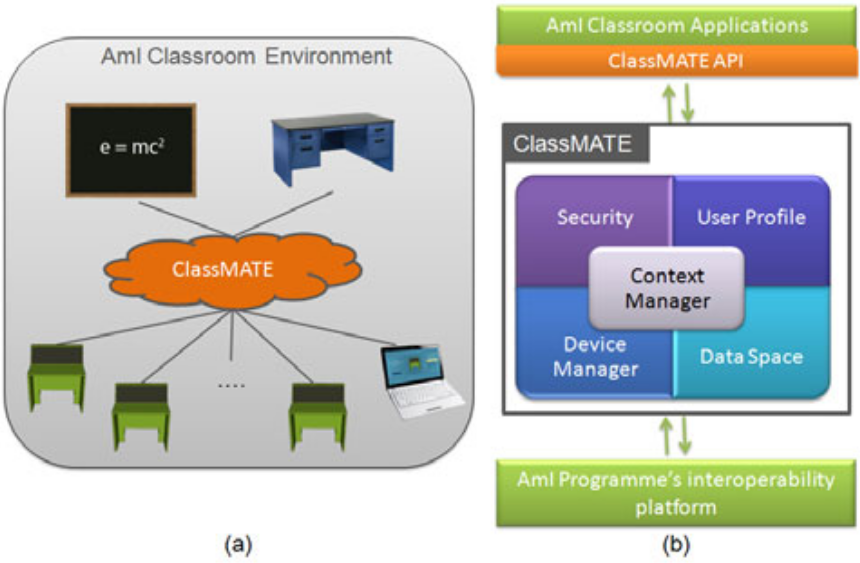
\includegraphics[width=0.8\linewidth]{imgs/margetis2011}
\caption{(a) Cenário do ClassMATE. (b) Arquitetura do ClassMATE}
\label{fig:margetis2011}
\end{figure}

\cite{Chang:2014} apresentam soluções de transformação de salas de aula tradicionais em salas de aula inteligentes baseadas em Internet das Coisas (IoT). Apresentam a definição de uma estrutura IoT composta por quatro camadas: \textit{Perceptive Layer, Network Layer, Processing Layer, Application Layer}. Afirma que há uma relação entre essas camadas e uma sala de aula. Assim, para tornar uma escola tradicional uma escola inteligente é necessário atingir três pontos:

\begin{enumerate}
   \item "Transformar uma sala de aula tradicional em uma IoT-base" através da instalação de um Set-top-box (STB) com webcam, RFID, Wifi e outras ferramentas de transmissão de dados (Figura~\ref{fig:chang2014}).
   \item Analisar o comportamento de aprendizagem dos alunos usando o RFID instalado no STB para identificar individualmente a presença do aluno na sala, além de enviar informações das respostas dos exercícios no \textit{tablet} ou \textit{smartphone} para gerar estatísticas relativas ao desempenho e às dificuldades dos alunos em determinado conteúdo de uma disciplina;
   \item Gerenciar dispositivos inteligentemente usando \textit{tablet} se comunicando através de Zigbee\footnote{Tecnologia de comunicação sem fio desenvolvida pela \textit{Zigbee Alliance} como padrão global aberto visando baixos custo e consumo de energia~\citep{Digi:2017}} para controlar dispositivos como projetor, ventilador, ar-condicionado e luzes.
\end{enumerate}

Ao detalhar os componentes de cada um desses pontos, o artigo apresenta em qual camada IoT um componente específico está localizado.

\begin{figure}[ht]
	\centering
	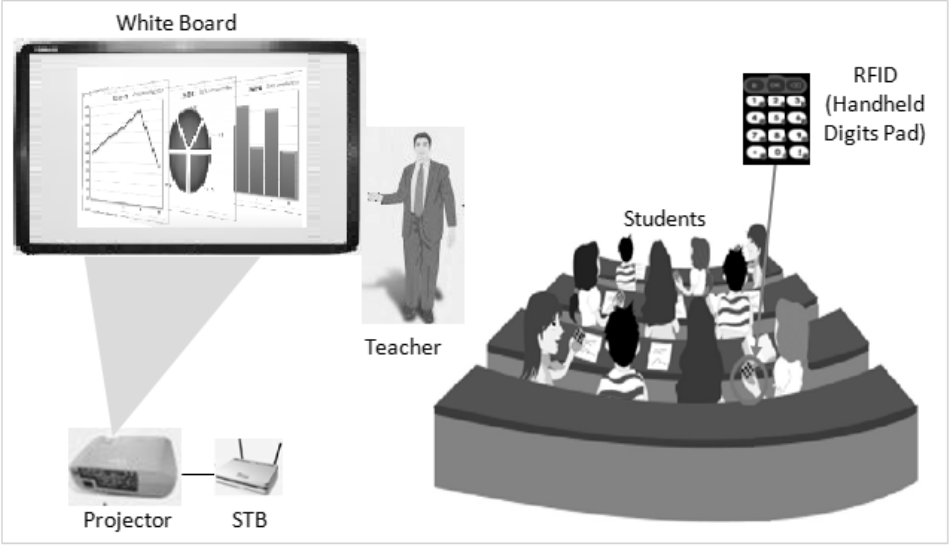
\includegraphics[width=0.8\linewidth]{imgs/Chang2014}
	\caption{Cenário de Sala de Aula Inteligente}
	\label{fig:chang2014}
\end{figure}

\cite{Savvaki:2013} apresentam o projeto de uma nova mesa (desk) para estudantes em uma sala de aula inteligente. A nova configuração utiliza como requisitos de projeto elementos de Estética, Usabilidade, Tecnologia e Viabilidade. Inicialmente, foram projetadas quatro alternativas baseadas no uso de tablet, mas, a versão final propõe um computador \textit{all-in-one} embarcado em uma estrutura que também permite atividades baseadas em papel (Figura~\ref{fig:Savvaki2013}). Duas mesas adjacentes podem se conectar e possibilitar atividades colaborativas e, assim, promover trabalhos em equipe.

\begin{figure}[ht]
\centering
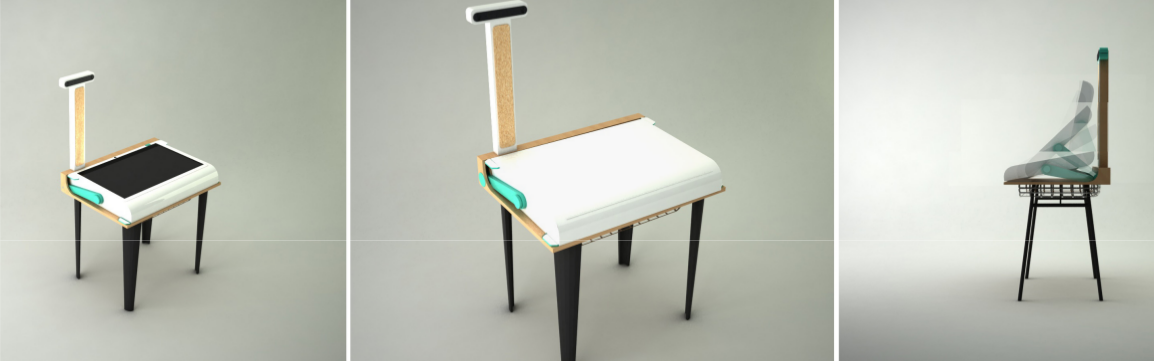
\includegraphics[width=0.9\linewidth]{imgs/Savvaki2013}
\caption{Mesa de estudos inteligente}
\label{fig:Savvaki2013}
\end{figure}

O trabalho de \cite{Zhang:2003} foca em aprendizado remoto que utiliza: protocolo multicast híbrido aplicação-camada, um software dedicado chamado "\textit{SameView}", uma sala de aula inteligente que é uma sala de aula ampliada com telas do tamanho da parede, sensores, câmeras e módulos de percepção e computação associados, alguns tipos de tecnologia de computação de padrões de aprendizagem, aprendizagem de interconexão através de protocolos de comunicação com e sem fio. A ideia é proporcionar maior participação na aula para quem está assistindo remotamente.

\cite{Mathioudakis:2013} apresentam uma abordagem centrada no aluno para dar apoio aos professores na melhoria do processo de aprendizado em ambientes educacionais. O sistema proposto apresenta uma infraestrutura multiagente inteligente que monitora, discretamente, as atividades dos alunos e notifica o professor, em tempo real, sobre as potenciais deficiências e armadilhas que precisam ser tratadas. O trabalho também aborda a questão da identificação do comportamento e análise de estatística de sala de aula.

O trabalho de \cite{Hwang:2009} está contextualizado no ensino da prática de laboratório de Difracção de Raios X de cristal único para pesquisadores inexperientes. O sistema identifica em que parte do laboratório o estudante está e, assim, infere a atividade que será executada por ele. Associando essa informação de contexto à temperatura ambiente, o estudante recebe instruções dos procedimentos que devem ser feitos, por exemplo, a seleção de um cristal de qualidade e tamanho adequado para a atividade a ser feita. Essas instruções são passadas através de um PDA (\textit{Personal Digital Assistant}). A efetividade do sistema foi medida através de pesquisa de opinião com os próprios estudantes que relataram uma melhoria no desempenho e na praticidade das aulas de laboratório.

Para \cite{Santana:2013}, simplesmente utilizar dispositivos móveis em sala de aula não é suficiente, é necessário que esses dispositivos se comuniquem entre si e contribuam com a melhoria do processo de ensino-aprendizagem. Este trabalho descreve a aplicação do conceito de Inteligência de Ambientes para criação de um ambiente educacional adaptado e personalizado, no caso, em escolas mexicanas. Foram utilizadas duas placas (mestre e escrava). A placa mestre (com um microcontrolador Pic18f4550) é a responsável pela interação com a sala de aula inteligente, monitoramento de temperatura, quantidade de luz ambiente, presença do professor para ligar o projetor e um \textit{display LCD} para monitoramento de todos os componentes. Entretanto, nada é explicitamente dito sobre o funcionamento da placa escrava.

\cite{Dekdouk:2012} introduz um ambiente de sala de aula inteligente baseado em "\textit{mobile learning}"~com uso de \textit{tablets}, \textit{RFID} e servidor de gerenciamento do ambiente (\textit{WebCT/Moodle}) focado na interação do estudante com o conteúdo (exemplo de aula de física) através do tablet e de uma lousa inteligente (Figura~\ref{fig:Dekdouk2012}). Nesse ambiente, também é possível fazer trabalhos em grupos. O trabalho apresenta um cenário e um esboço de um protocolo de comunicação, entretanto, não são executados testes e não é feito reconhecimento de atividades ou comportamentos.

\begin{figure}[ht]
	\centering
	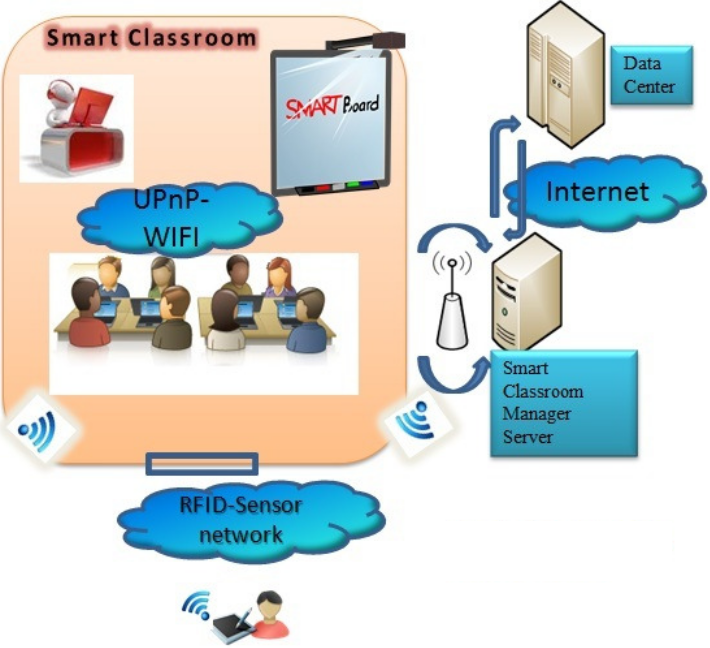
\includegraphics[width=0.6\linewidth]{imgs/Dekdouk2012}
	\caption{Sala de aula inteligente}
	\label{fig:Dekdouk2012}
\end{figure}

\cite{Gligoric:2012} apresentam um sistema de inferência da qualidade de uma palestra com ênfase na aplicação de Internet das Coisas (IoT) em Sala de Aula Inteligente. Neste trabalho é discutido como Inteligência de Ambientes pode ser usada para oferecer um \textit{feedback} automático e em tempo real da qualidade de uma palestra em auditório baseando-se em parâmetros. Utilizando sensores de ruído, \textit{Passive Infrared} (PIR), câmeras de vídeo e microfones. A inferência da qualidade da palestra é feita a partir do nível de interesse da plateia, que pode ser medido pela inquietação dos ouvintes e pelo ruído ambiente. 


% Após apresentados e discutidos alguns pontos dos trabalhos correlatos que abordam a construção de ambientes de internos de aprendizagem, nota-se que a abordagem proposta nesta dissertação se diferencia das pesquisas relacionadas expostas até o momento, especialmente no que diz respeito à materialidade do ambiente proposto. Nesta dissertação, trabalha-se igualmente na construção de um ambiente baseado em sala de aula presencial, mas, não se mantém o foco unicamente na construção de novos dispositivos ou aparatos físicos, como os trabalhos apresentados nesta Seção~\ref{section:wIndoorClassroom}. A maior parte das intervenções contidas no método proposto nesta dissertação, diz respeito à inserção de tecnologia usando o conceito de computação pervasiva, de modo que, a interação das pessoas com os dispositivos seja percebida como algo natural. Por isso, os diversos elementos de intervenção direta no ambiente de sala de aula propostos neste trabalho primam por utilizar equipamentos já existentes e muito utilizados no dia a dia, tais como, computadores pessoais, \textit{smartphones} e \textit{tablets}. Sendo assim, no sentido de construção de ambiente de sala de aula, a abordagem proposta tem também baixo custo de implantação, uma vez que é possível utilizar uma infraestrutura pré-existente em diversas escolas.

% % -----------------------------------------------------------------
% => Ambiente Externo
% -----------------------------------------------------------------

\subsection{Ambiente Externo de Aprendizagem}
\label{section:OutdoorClassroom}

\cite{Xue:2011} descrevem um \textit{framework} para criação de ambiente de aprendizado ubíquo baseado em Internet das Coisas e com três camadas: percepção, rede de computadores e aplicação. Apesar de não utilizar um sensor específico, este trabalho indica elementos que podem ser utilizados para construir um ambiente de aprendizado ubíquo e que seja integrado com qualquer sensor ou aplicação (Figura~\ref{fig:Xue2011}).

\begin{figure}[ht]
	\centering
	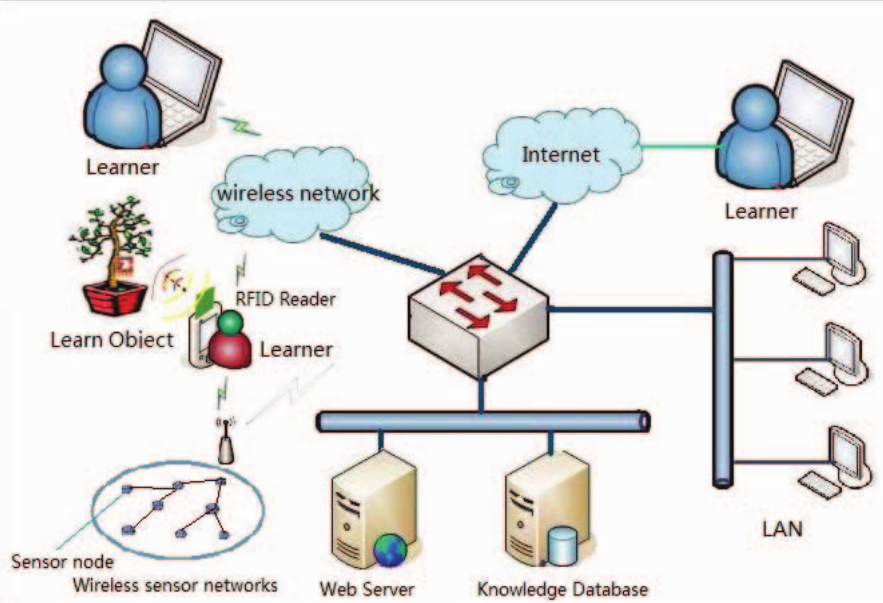
\includegraphics[width=0.9\linewidth]{imgs/Xue2011}
	\caption{Arquitetura do Sistema de Aprendizagem Ubíqua}
	\label{fig:Xue2011}
\end{figure}

\cite{Oluwagbemi:2014} apresentam uma revisão de literatura acerca das tendências da aplicação de métodos de computação pervasiva em ambientes de sala de aula apresenta trabalhos focados em \textit{3D Printing}, \textit{Quantified Self}, Assistentes Virtuais, Jogos e \textit{Gamification}. Como trabalhos futuros é sugerida a adoção e implementação de um modelo nigeriano de ambiente de aprendizado em sala de aula.

\cite{Dong:2007} apresentam um método de reconhecimento de contexto de aprendizagem baseado na Análise do Comportamento para recomendação de um calendário de estudos, quando o estudo é feito em casa, com o objetivo de incentivar o estudante a adquirir o hábito da aprendizagem. O trabalho utiliza sensores de RFID para detectar se os livros estão sobre a mesa de estudo e o sistema cruza essa informação com os dados dos professores e a demanda dos pais para considerar se o aluno está ou não em um contexto de aprendizagem. Se estiver, então, uma programação de estudos é feita pelo sistema. Entretanto, a avaliação do desempenho do sistema foi feita através de formulários aplicados aos estudantes, onde mais de 80\% concordou que o sistema proposto contribui para a melhoria do processo de aprendizado.

\cite{Tan:2007} propõem utilizar a tecnologia em ambientes de aprendizagem externa para ajudar num maior ganho educacional. Utilizando os conceitos de aprendizagem móvel, aprendizagem ubíqua e reconhecimento de contexto foi desenvolvido um sistema denominado "\textit{Ubiquitous Learning with Educational Resources}"~(EULER) baseado em RFID, Internet, redes sem fio, sistemas embarcados e tecnologias de Banco de Dados.

\begin{figure}[ht]
	\centering
	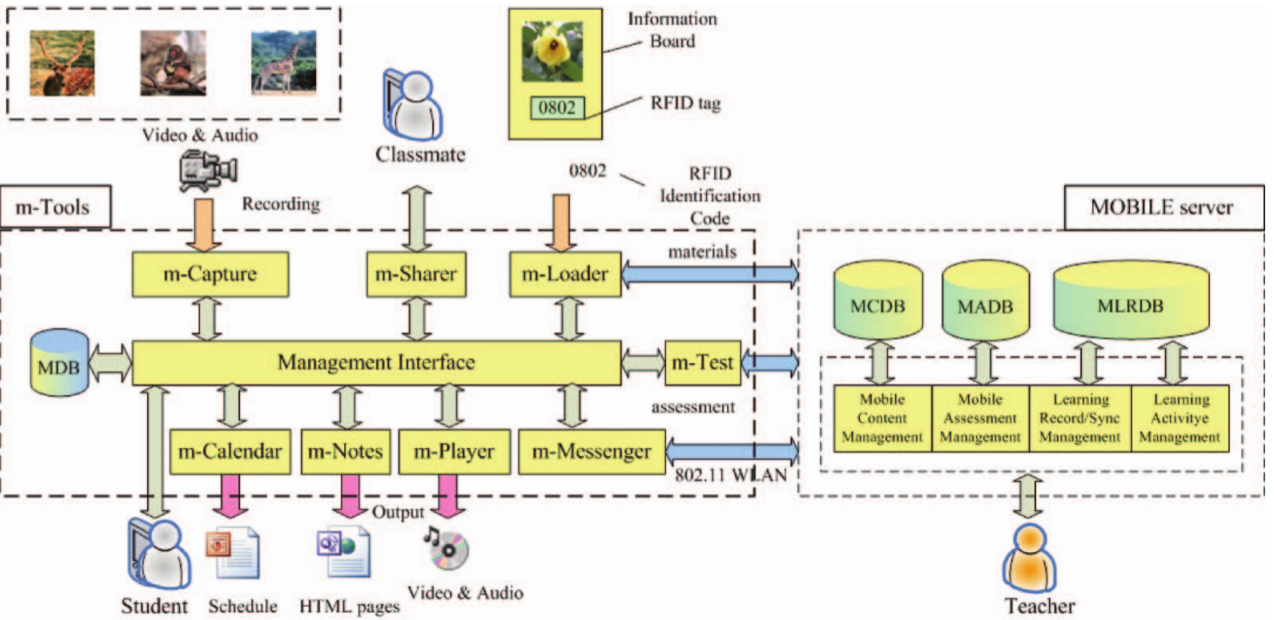
\includegraphics[width=0.8\linewidth]{imgs/Tan2007a}
	\caption{Estrutura do sistema EULER}
	\label{fig:Tan2007a}
\end{figure}

O sistema EULER consiste em dois subsistemas (Figura~\ref{fig:Tan2007a}): (a) Servidor "\textit{MObile-Based Interactive Learning Environment}"(MOBILE) para uso do professor; (b) ferramentas móveis para os estudantes (m-Tools). O professor prepara e armazena o material didático (que pode conter temas, imagens, áudios e descrição textual) no servidor, construindo as relações entre este e os códigos RFID. Os alunos podem coletar e compartilhar dados, além de editar artigos ao seu próprio critério. Dentre as ferramentas do \textit{m-Tools} que os estudantes podem usar estão: PDA, leitor RFID e câmera.

Com tudo configurado, a aula pode acontecer em qualquer ambiente externo, seja um museu, um zoológico ou um parque. A Figura~\ref{fig:Tan2007b} apresenta um cenário de uso do EULER no \textit{Guandu Nature Park} em Taiwan.

\begin{figure}[ht]
	\centering
	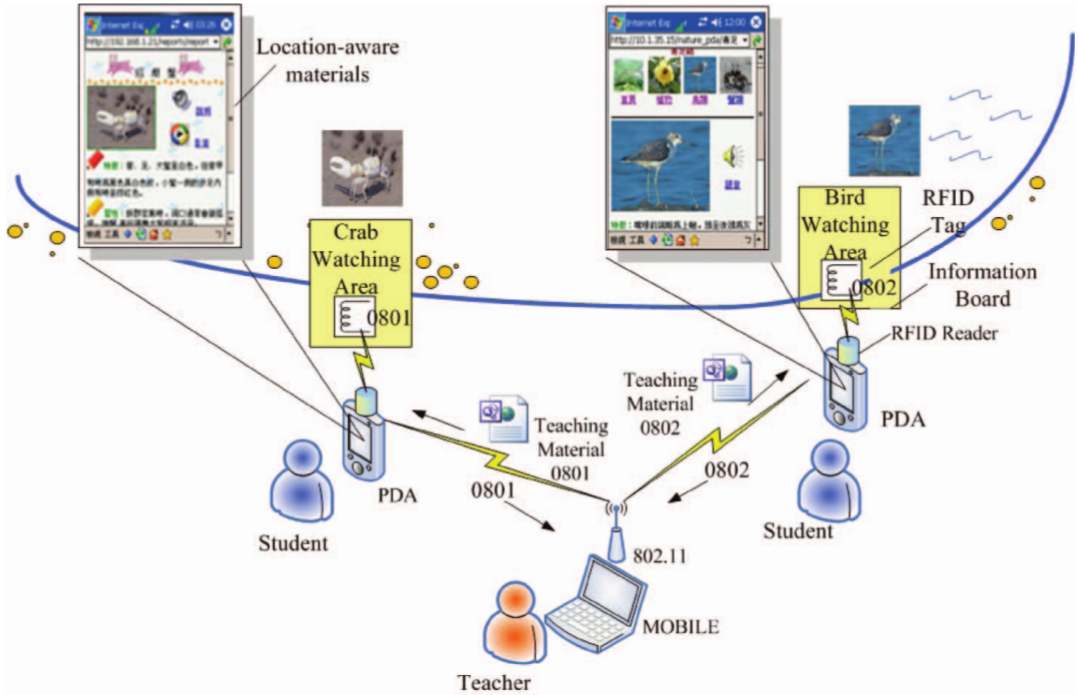
\includegraphics[width=0.9\linewidth]{imgs/Tan2007b}
	\caption{Cenário de uso do sistema EULER no Guandu Nature Park}
	\label{fig:Tan2007b}
\end{figure}

Os experimentos foram executados com dois grupos de 36 alunos cada e o auxílio de quatro professores experientes em educação com uso de computadores. Um grupo experimental utilizou o EULER e um grupo de controle recebeu instrução tradicional. Os experimentos foram divididos em quatro fases e foram aplicados testes antes, durante e depois dos experimentos, com exceção do pré-teste, os estudantes que utilizaram o EULER obtiveram maior desempenho em todos os testes das quatro fases.

% Após breve apresentação e discussão dos trabalhos correlatos à construção de ambientes externos de aprendizagem, nota-se que a abordagem proposta nesta dissertação tem grande proximidade, a maior parte desses trabalhos faz uso de metodologias de aprendizado ubíquo que permitem que a interação do estudante com o sistema seja a mais natural possível, mesmo em ambientes não controlados, como um museu ou um parque.

% É importante observar que, tanto os trabalhos voltados à construção de ambientes internos de aprendizagem, quanto os trabalhos que propõe metodologias para ambientes externos não apresentam: (i) ferramentas de apoio ao professor na fase de composição da aula; (ii) inserção de metodologias de ajuda sob demanda, especialmente, voltadas para a avaliação da aprendizagem dos estudantes; (iii) métricas de aprendizagem para análise \textit{a posteriori} do desempenho dos estudantes após a execução de uma aula. Outro fator importante consiste de que a maior parte dos trabalhos que fazem alguma análise de desempenho, voltam-se para avaliação do sistema baseada unicamente em formulários de opinião aplicados aos estudantes. A proposta apresentada neste trabalho é avaliada utilizando métricas de aprendizagem que possibilitem ao professor fazer análises, inferências e, assim, tomar decisões que impactem positivamente o desempenho dos estudantes. Desse modo, a eficácia do método proposto neste trabalho está ligada à sua capacidade de apresentar métricas que permitam ao professor fazer um diagnóstico da turma para tomadas de decisões relacionadas às metodologias utilizadas durante a execução da aula.

% %Achei que antes do resumo faltou você comentar (pode ser em um parágrafo) em que aspectos o teu trabalho vai acrescentar o estado-da-arte, principalmente quando comparado com os trabalhos correlatos.

\section{Ferramentas de Autoria de Objetos de Aprendizagem}
\label{sec:autoria}
%\label{section:author_performance_evaluation}

Ferramentas de autoria auxiliam nos processos de criação, inserção e utilização de objetos de aprendizagem como parte do material didático com o objetivo de facilitar o ensino-aprendizagem e, assim, contribuir com o engajamento e a construção do conhecimento por parte dos estudantes. Neste trabalho, o processo de autoria de objetos de aprendizagem, especialmente questionários avaliativos e objetos tangíveis, está a cargo do módulo Compositor (ver Seção \ref{section:composer}), de modo que esta seção apresenta alguns trabalhos relacionados a métodos e ferramentas de autoria.

Tendo em vista que pacotes de aplicativos para escritório contendo editores de texto, de planilhas ou de apresentação são amplamente difundidos e que, por isso, tais ferramentas podem ter seu uso facilmente direcionado para a criação de objetos de aprendizagem, \cite{Passos:2010} propõem a inserção de códigos em VBA (\textit{Visual Basic for Applications}) no Microsoft PowerPoint para criação de aplicações interativas que facilitem a aprendizagem dos conteúdos curriculares em escolas públicas de um município do interior do Estado do Amazonas~(Brasil).

\begin{figure}[htb]
	\centering
	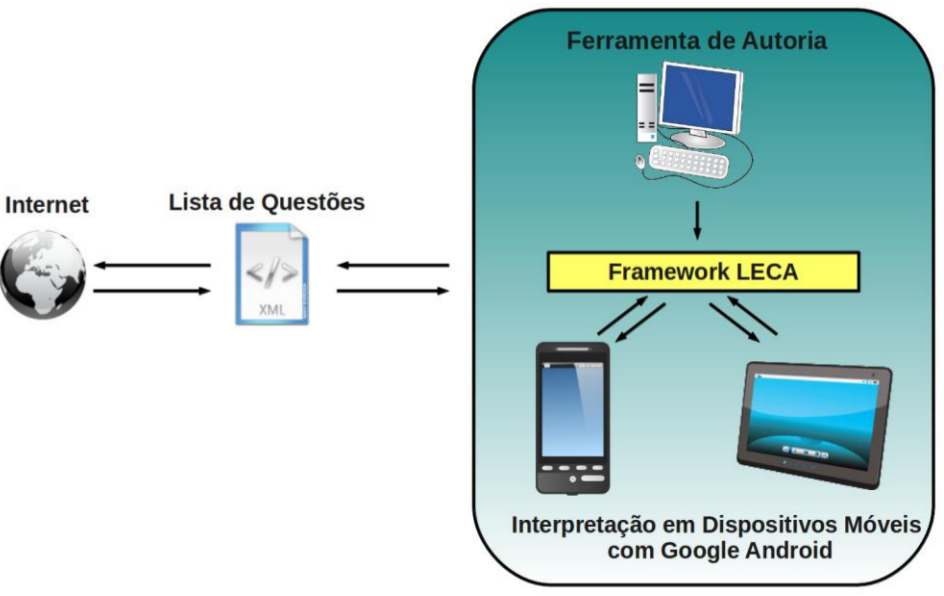
\includegraphics[width=0.8\linewidth]{chapters/works/orlandi2012.png}
	\caption{Arquitetura do LECA. Fonte:~\cite{Orlandi:2012}}
	\label{fig:orlandi2012}
\end{figure}

\cite{Orlandi:2012} apresentam uma ferramenta de autoria para dispositivos móveis chamada LECA (Lista de Exercícios com Correção Automática), focada na criação e na responsividade de listas de exercícios de múltipla escolha com avaliação do desempenho do aluno através de pontuação. A Figura~\ref{fig:orlandi2012} apresenta o diagrama da relação do \textit{framework} do LECA com as aplicações diversas, onde nota-se que o sistema é composto por uma parte de autoria das questões e por outra de visualização.

\begin{figure}[htb]
	\centering
	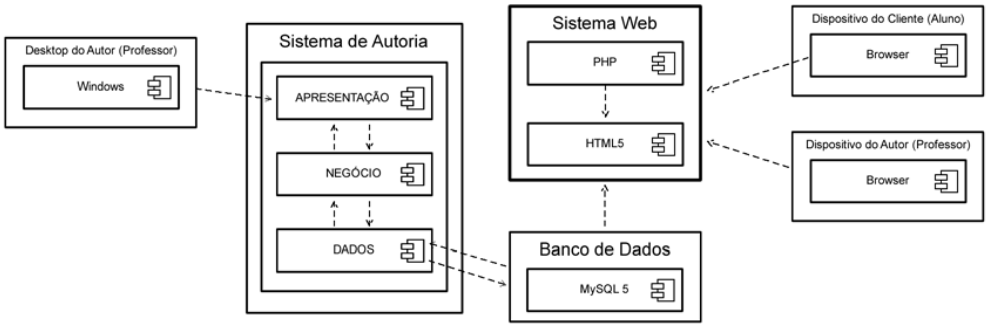
\includegraphics[width=0.8\linewidth]{chapters/works/guterres2014.png}
	\captionsetup{justification=centering}
	\caption{Estrutura da Plataforma ``Fábrica de Objetos''. \\Fonte:~\cite{Guterres:2014}}
	\label{fig:guterres2014}
\end{figure}

\cite{Guterres:2014} descrevem uma plataforma para construção de objetos de aprendizagem com foco em usuários com pouco conhecimento de informática. A plataforma apresentada foi implementada usando tecnologias web, dentre elas: HTML5, CSS e JQuery. A Figura~\ref{fig:guterres2014} ilustra o diagrama de componentes desta plataforma, onde pode-se observar que ela tem duas partes principais: (a) Sistema de Autoria e (b) Sistema Web com Banco de Dados. Onde o Sistema de Autoria é o responsável de fato pela criação, modificação ou remoção dos objetos de aprendizagem ou das páginas que os compõem e o Sistema Web permite o gerenciamento destes OAs. Além disso, cada objeto de aprendizagem existente no repositório é organizado conforme ilustrado na Figura~\ref{fig:guterres2014_objetos}.

\begin{figure}[htb]
	\centering
	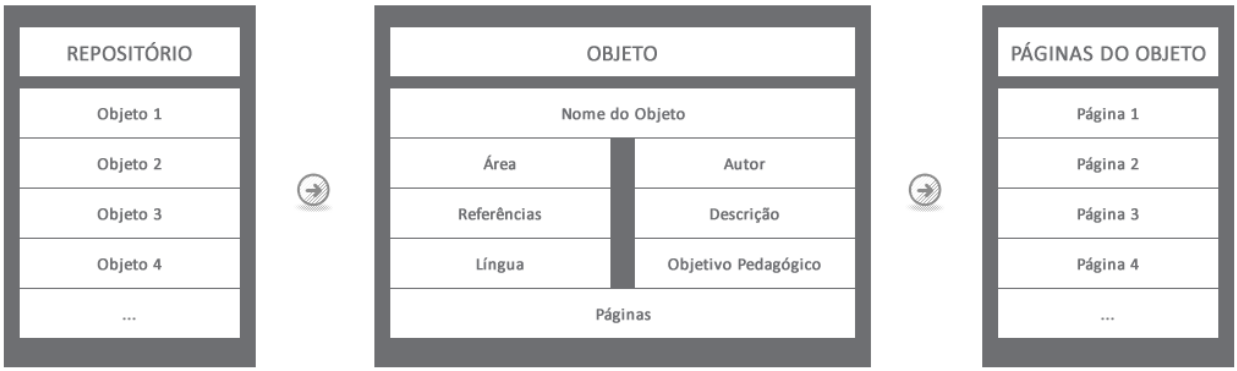
\includegraphics[width=1\linewidth]{chapters/works/guterres2014_objetos.png}
	\captionsetup{justification=centering}
	\caption{Estrutura dos OAs na plataforma ``Fábrica de Objetos''. \\Fonte:~\cite{Guterres:2014}}
	\label{fig:guterres2014_objetos}
\end{figure}


%\cite{Flores:2011}, baseando-se em Kolb, Gagné e Wiley, definem um conjunto de funcionalidades que precisam estar presentes em uma ferramenta de autoria para a construção de objetos de aprendizagem mais adequados. Além disso, apresentam um exemplo de criação e aplicação de um objeto de aprendizagem para ensino de matemática usando a ferramenta gratuita eXeLearning. Dentre as funcionalidades descritas no artigo, destacamos: \textit{Applet Java}, Apresentação em \textit{Slides}, Textos, Imagens, Questionários de múltipla escolha ou verdadeiro-falso, entre outros.

\section{Ferramentas e Métricas de Avaliação do Desempenho}\label{sec:avaliacao}
%\label{sec:related-avaliacao-aprendizagem}

As novas tecnologias possibilitam obter dados de interação dos estudantes ao longo do processo de aprendizagem, permitindo gerar gráficos e análises que auxiliem o professor na avaliação e na tomada de decisões que envolvam, por exemplo, a adição de atividades pedagógicas que reforcem o aprendizado de um conteúdo, e é considerada uma estratégia pedagógica mais eficiente.
Assim, dados obtidos de aulas e avaliações podem permitir melhores inferências relacionadas ao perfil de aprendizagem e às dificuldades de uma determinada turma ou de um único estudante. Desta forma, o sistema pode recomendar diversas atividades e estratégias que sejam mais adequadas e adaptadas às reais necessidades da classe ou aluno.

Além disso, há ainda pesquisas relacionadas ao desenvolvimento de métricas e ferramentas específicas para a avaliação do desempenho dos estudantes a fim de melhorar o acompanhamento da aprendizagem por parte do professor. 
Assim, esta seção apresenta alguns trabalhos correlatos a avaliação da aprendizagem de estudantes em situação escolar.

%Avaliação do desempenho
%\cite{Malvezzi:2010} introduzem uma ferramenta para avaliação de alunos em cursos presenciais mediados por tecnologia aplicando a Teoria \textit{Fuzzy} em variáveis de interação como \textit{chat}, fórum, tarefas e testes. 

\subsection{WebMonitor - monitoramento e acompanhamento}
\cite{Lucena:2015} propõem uma ferramenta para monitoramento de desempenho em um Ambiente Virtual de Aprendizagem (AVA) chamada o WebMonitor, que funciona como um \textit{plugin} para monitoramento de \textit{logs} de tarefas e participação em fóruns do Moodle.

\begin{figure}[htb]
	\centering
	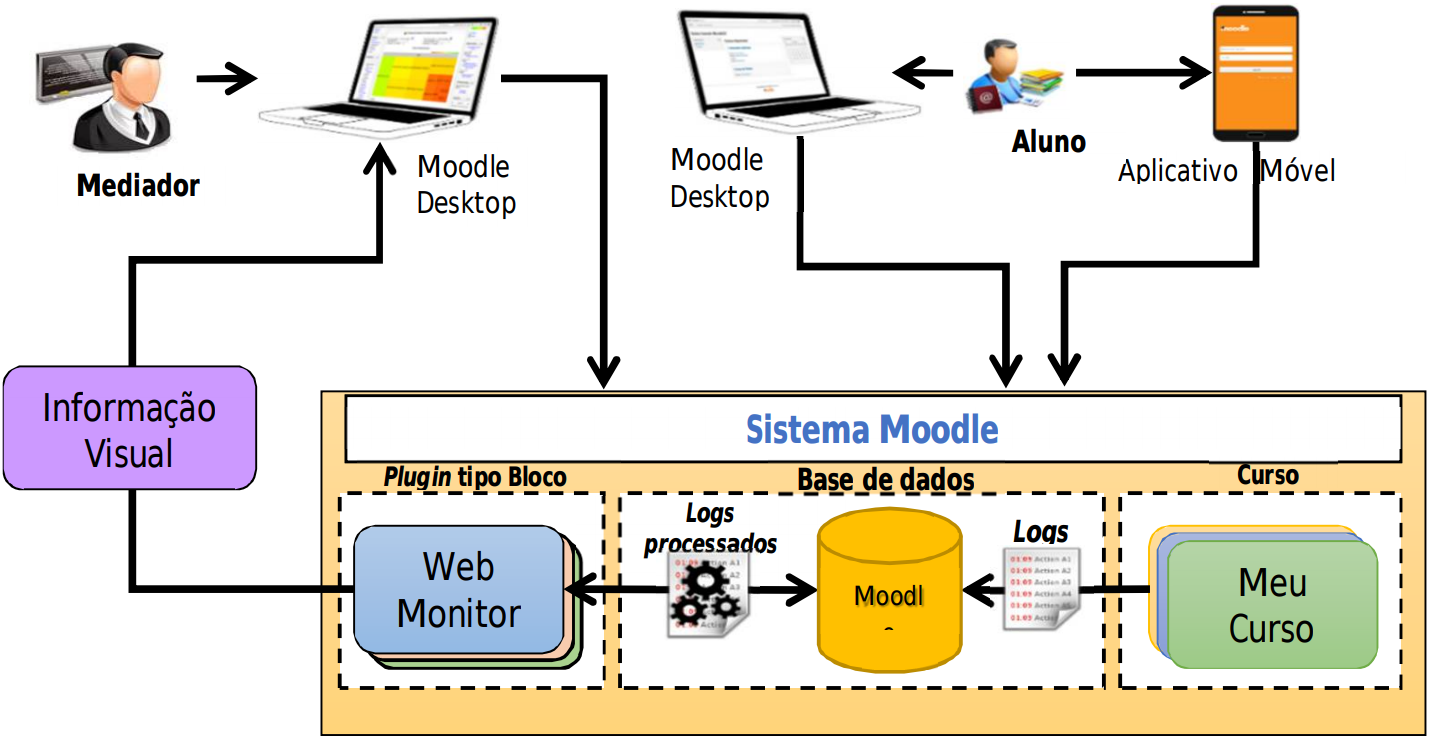
\includegraphics[width=0.9\linewidth]{chapters/works/Lucena2015_5162-6882-1-PB_arquitetura.png}
	\caption{Arquitetura do WebMonitor. Fonte:~\cite{Lucena:2015}}
	\label{fig:Lucena2015_Arquitetura}
\end{figure}

A Figura~\ref{fig:Lucena2015_Arquitetura} apresenta a arquitetura da ferramenta, cujo fluxo de informações pode ser resumido em cinco passos~\citep{Lucena:2015}: 
\begin{enumerate}
    \item Acesso ao AVA Moodle pelos estudantes (via Desktop ou dispositivo móvel);
    \item Moodle coleta as ações dos usuários e as registra em um log;
    \item Mediador acessa o WebMonitor instalado no Moodle;
    \item WebMonitor recupera e processa os dados de logs da base de dados do Moodle;
    \item A informação processada é transformada visualmente e disponibilizada ao mediador através de representações gráficas (\textit{Treemaps} e gráficos de barras).
\end{enumerate}

Desse modo, o monitoramento é realizado utilizando a técnica \textit{Treemap} para visualização da informação a fim de auxiliar o professor na percepção do desempenho acadêmico e do comportamento dos estudantes em atividades como postagem de arquivos e interações em fóruns de discussão, o que, segundo os autores, possibilitaria melhores condições de identificar possíveis desistências, reprovações ou evasão de
estudantes por parte dos professores ou mediadores. Na Figura~\ref{fig:Lucena2015}, o WebMonitor exibe as interações de um aluno.

\begin{figure}[htb]
	\centering
	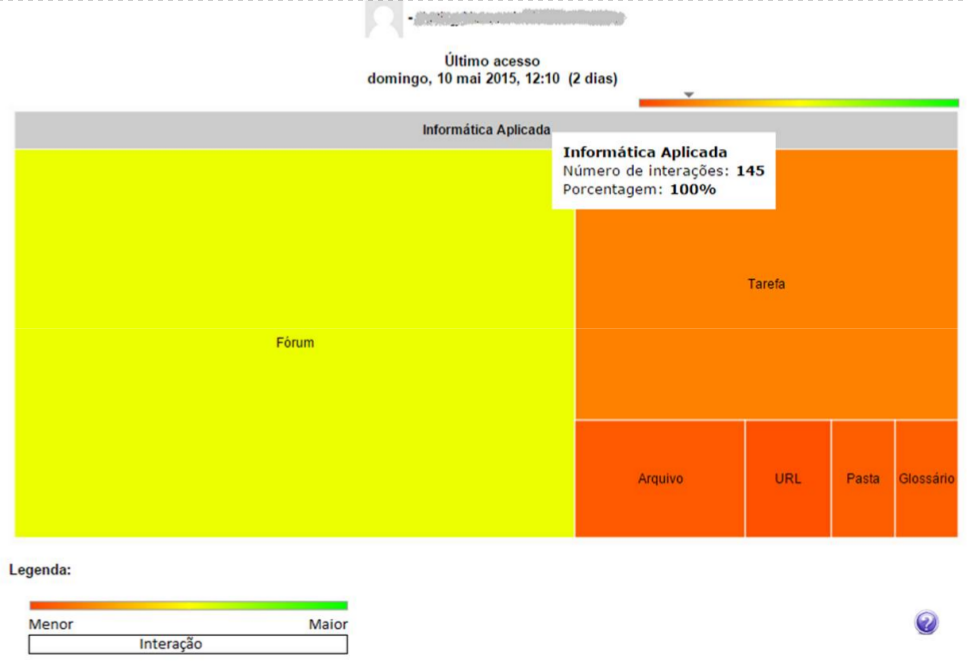
\includegraphics[width=0.9\linewidth]{chapters/works/Lucena2015.png}
	\captionsetup{justification=centering}
	\caption{Exemplo do Treemap das interações de um estudante. \\Fonte:\cite{Lucena:2015}}
	\label{fig:Lucena2015}
\end{figure}

\subsection{Metodologia para \textit{Learning Analytics}}

Com enfoque em cursos semipresenciais ou híbridos, \cite{Nunes:2016} propõem uma metodologia de avaliação onde o desempenho é calculado a partir das notas e da participação do aluno. 

De acordo~\cite{Nunes:2016}, o processo de \textit{Learning Analytics} consiste nos cinco passos seguintes: (1) Capturar dados; (2) Reportar dados; (3) Predizer; (4) Adaptar; (5) Personalizar; e (6) Intervir. Além disso, as técnicas utilizadas para a realização de \textit{Learning Analytics} podem ser: (i) análises de redes sociais; (ii) processamento de linguagem natural; (iii) predição; (iv) determinação de risco; (v) sequenciamento de curso; e (vi) identificação de alunos que precisam de ajuda.

Assim, a proposta apresentada por~\cite{Nunes:2016} apresenta como critério avaliativo, para cada aluno, o cálculo de uma Nota Final (NF), a partir da Equação~\ref{equacao:nunes2016}. Onde, PT é dada pela ``Participação da Turma'', seja virtual (fóruns, mensagens e \textit{chats}), seja presencial (assiduidade, resolução de exercícios em sala, cumprimento de prazos de entrega); AE são ``Atividades Executadas'' e PE é a nota da ``Prova Escrita''. 

Como \textit{feedback}, são apresentados gráficos de quantidade de alunos aprovados e reprovados por turma (Figura~\ref{fig:Nunes2016}), relação entre a nota da participação virtual ou presencial e o número de acessos por turma.

\begin{equation}\label{equacao:nunes2016}
NF = \frac{(PT + AE + (PE*2)}{4}
\end{equation}

\begin{figure}[htb]
	\centering
	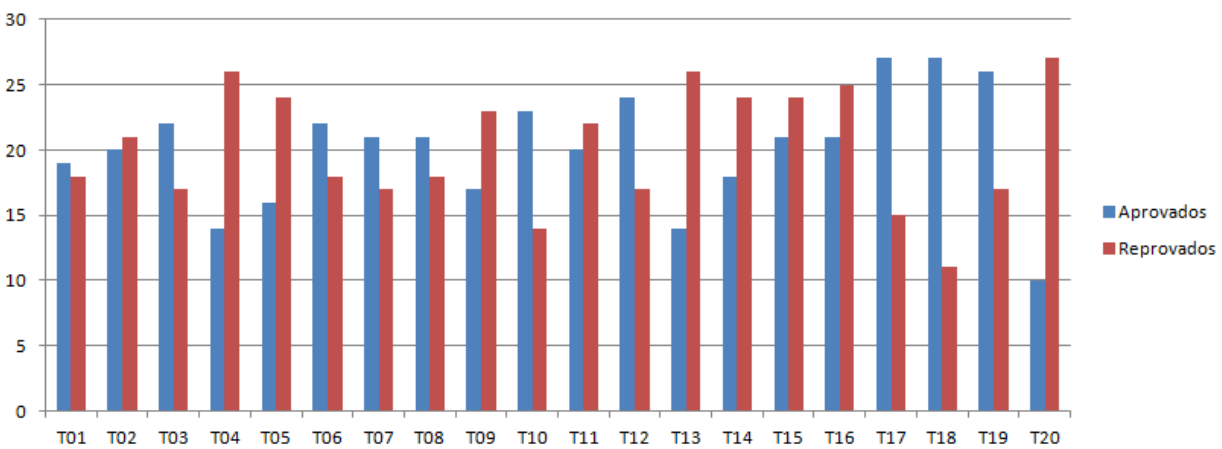
\includegraphics[width=1\linewidth]{chapters/works/Nunes2016.png}
	\captionsetup{justification=centering}
	\caption{Alunos Aprovados e Reprovados por Turma}
	\label{fig:Nunes2016}
\end{figure}

\subsection{Métricas de Desempenho para Estudantes e Professores}
\label{sec:level-understanding}

Um conjunto de métricas que leva em consideração o histórico de atividades dos estudantes foi descrito por~\cite{Biswas:2007}, são eles: (a) Nível de Compreensão, (b) Taxa de Aprendizagem do Aluno e, (c) Nível de dificuldade de um elemento de ontologia (assunto, tópico ou conceito).

\textbf{Nível de Compreensão (Equação~\ref{eq:lu})} é uma métrica que quantifica a relação entre diferentes índices de dificuldade, tempo de resposta e desvio. Os \textbf{índices de dificuldade} (tópico, conceito e questão) são descritos na Tabela~\ref{tab:Lu}.
O \textbf{tempo de resposta} é aplicado para capturar os chutes do estudante e deve ser comparado com o tempo de resposta esperado fornecido pelo autor da questão. Existem duas classes de Tempo de Resposta, a classe ``chute'' com valor 5 e a ``resposta normal'' (ou opinião fundamentada), cujo valor é 1.
O parâmetro \textbf{desvio} é dado de acordo com a classificação de resposta mostrada na Tabela ~\ref{tab:Weight_Biswas}, onde 0 significa que é uma resposta ``completamente incorreta'' e 5 corresponde a resposta ``perfeita'', ou seja, a resposta correta.

\begin{equation}\label{eq:lu}
L_u = \frac{IDT \cdot IDC \cdot IDQ \cdot Desvio}{Tempo \ de \ Resposta}
\end{equation}

\begin{table}[htbp]
\centering
\caption{O índice de dificuldade significa o quão difícil é uma questão ou tópico.}
\begin{center}
\begin{tabular}{|l|c|c|c|}
\hline
\textbf{Índice de Dificuldade} & \textbf{Fácil} & \textbf{Normal} & \textbf{Difícil} \\\hline
Índice de Dificuldade do Tópico (IDT) & 1 & 3 & 5 \\\hline
Índice de Dificuldade do Conceito (IDC) & 1 & 3 & 5 \\\hline
Índice de Dificuldade da Questão (IDQ) & 1 & 3 & 5 \\\hline
\end{tabular}
\end{center}
\label{tab:Lu}
\end{table}

\cite{Biswas:2007} enfatizam que os valores das Tabelas~\ref{tab:Lu}, \ref{tab:Weight_Biswas} e do ``Tempo de Resposta'' não foram derivados matematicamente, mas eles são aplicados apenas para diferenciar as distintas classes de estudantes. Nesse caso, é possível escolher quaisquer outros valores.

\begin{table}[htbp]
\caption{Valor do parâmetro Desvio}
\centering
\begin{tabular}{|c|c|c|c|c|c|}
\hline
\textbf{Desvio} & \textbf{Não tem ideia} & \textbf{Abaixo do Meio} & \textbf{Meio} & \textbf{Quase correto} & \textbf{Correto} \\ \hline
\textbf{Valor} & 0 & 2 & 3 & 4 & 5\\ \hline
\end{tabular}
\label{tab:Weight_Biswas}
\end{table}

Para estabelecer a métrica \textbf{Taxa de Aprendizado do Estudante ($SLR$)}, \cite{Biswas:2007} introduzem a definição de ``Pontuação do Estudante'', definida por $SS (s,i,o)$, que diz sobre a pontuação de um estudante $s$ em uma $i$-ésima avaliação em relação a um elemento ontológico $o$, onde esta ontologia pode ser uma disciplina, tópico ou conceito.
Assim, a taxa de aprendizado do estudante é a melhoria, na média, na pontuação de um estudante com respeito ao conjunto de avaliações. Isso permite a observação da evolução contínua e é expressa pela Equação~\ref{eq:student_rate}, onde $N$ é o total de questões acerca do elemento ontológico $o$, e $i$ é uma variável que expressa uma avaliação específica.

\begin{equation}\label{eq:student_rate}
\begin{split}
SLR(s,o) =  \frac{\sum \{(SS(i+1)-SS(i)) \cdot |SS(i+1)-SS(i)| \} }{N-1}
\end{split}
\end{equation}

%\noindent onde $N$ é o total de questões acerca do elemento ontológico $o$, e $i$ é uma variável que expressa uma avaliação específica.

Finalmente, \cite{Biswas:2007} definem que o \textbf{Nível de Dificuldade ($DL$)} de um elemento ontológico $o$ pode ser quantificado para todo $s$ através da Equação~\ref{eq:DL}.

\begin{equation}\label{eq:DL}
DL(o) = \overline{SLR}(s,o)
\end{equation}

\subsection{Modelo \textit{Learning Vectors} para \textit{Moodle}}
\label{sec:learningvectors}

\begin{figure}[htb]
	\centering
	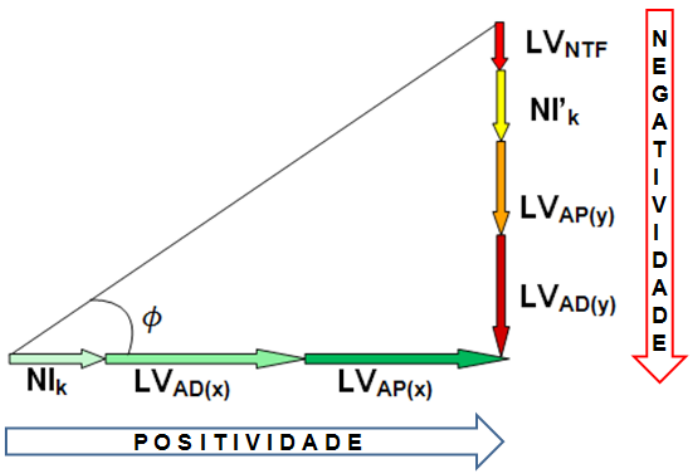
\includegraphics[width=0.45\linewidth]{chapters/works/Sales2019_LearningVectors_FatorB2.png}
	\caption{Representação do Vetor-Aprendizagem. Fonte:\cite{sales:2019}}
	\label{fig:Sales2019fatorbeta}
\end{figure}

\cite{sales:2019} apresentam uma ferramenta para Avaliação Formativa no AVA Moodle através de \textit{emoticons} e GIFs animados que alimentam um modelo baseado em Vetores-Aprendizagem. Os \textit{emoticons} e GIFs compõem uma escala iconográfica que os associa às seguintes menções qualitativas: ``muito bom'', ``bom'', ``regular'', ``fraco'', ``não satisfatório'' e ``neutro'' com o objetivo de alimentar um modelo matemático que leva em consideração as interações dos alunos em fóruns de discussão, tarefas, wikis e salas de chats para gerar pontuações, permitindo também a importação de notas de quizzes e o gerenciamento da frequência dos alunos.

A Figura~\ref{fig:Sales2019} apresenta o modelo proposto por~\cite{sales:2019}, onde, através de uma escala de menções qualitativas baseada na Escala Likert associada ao uso de \textit{emoticons} e GIFs, o professor/tutor avalia as interações dos alunos nas diversas atividades dentro do Moodle. Com essas avaliações, é possível calcular os vetores de aprendizagem (Figura~\ref{fig:Sales2019fatorbeta}) de modo que as projeções horizontais (LVx) e verticais (LV{y}) do vetor expressam, de um lado, a positividade de desempenho do aluno e a nota da atividade e, de outro, a negatividade do desempenho, respectivamente.

\begin{figure}[htb]
	\centering
	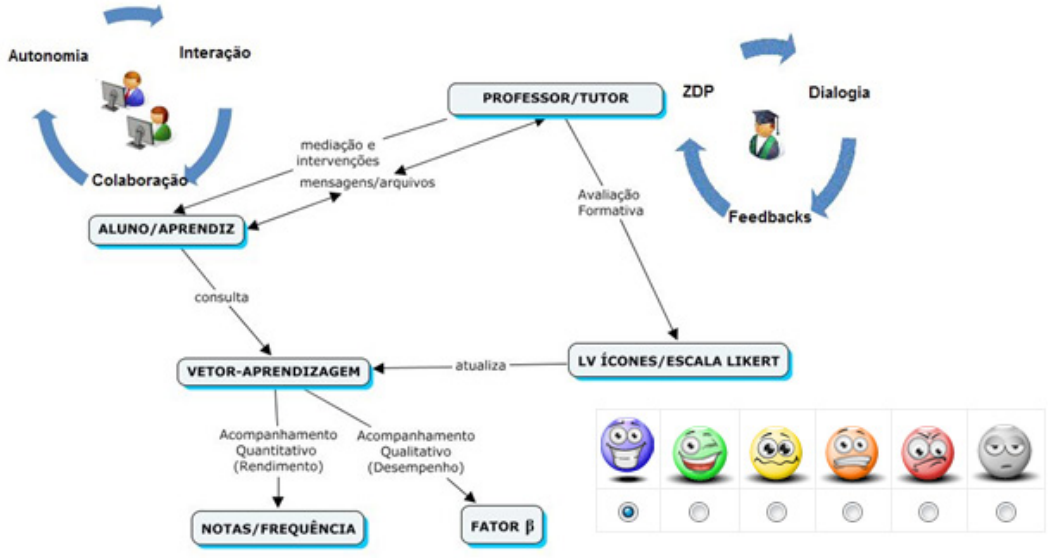
\includegraphics[width=1\linewidth]{chapters/works/Sales2019_LearningVectors.png}
	\captionsetup{justification=centering}
	\caption{Modelo de Avaliação usando Learning Vectors. \\Fonte:~\cite{sales:2019}}
	\label{fig:Sales2019}
\end{figure}

Além disso, em um trabalho anterior, \cite{sales:2012} especificam que a Positividade ($P$), dada pela Equação~\ref{eq:Positividade}, é o somatório das projeções horizontais dos vetores de aprendizagem $LV_{AD(x)}$ de atividades a distância (fóruns, chats, tarefas e wikis) e $LV_{AP(x)}$ de atividades presenciais, acrescido do número de interações positivas $NI_k$ ponderadas e categorizadas pelo professor/tutor como ``muito bom'' (peso 3 - azul), ``bom'' (peso 2 - verde) e ``regular'' (peso 1 - amarelo).

\begin{equation}
	\label{eq:Positividade}
	P = \sum_{x}^{i=1} LV_{ADi} +  \sum_{y}^{j=1} LV_{APj} + \sum_{z}^{k=1} NI_k
\end{equation}

Por sua vez, a Negatividade ($N$), expressa na Equação~\ref{eq:Negatividade}, é o somatório das projeções verticais dos vetores de aprendizagem $LV_{AD(y)}$ e $LV_{AP(y)}$, acrescido do somatório do número de interações negativas $NI'_k$ categorizadas como ``fraco'' (peso 1 - laranja) ou ``não satisfatório'' (peso 2 - vermelho) e do número total de faltas, dado por $LV_{NTF}$~\citep{sales:2012}.

\begin{equation}
	\label{eq:Negatividade}
	N = \sum_{x}^{i=1} LV'_{ADi} +  \sum_{y}^{j=1} LV'_{APj} + \sum_{z}^{k=1} NI'_k + LV_{NTF}
\end{equation}

Dados os vetores ortogonais de positividade e negatividade, é calculado o ``Fator $\beta$'', que é dado por $\nicefrac{P}{N}$ e é o indicador qualitativo não linear do nível de desempenho dos alunos~\citep{sales:2012}.

\section{Resumo}
Neste capítulo, descrevemos e analisamos diversos trabalhos relacionados com a criação e utilização de manipulativos físicos e virtuais no contexto educacional, tais trabalhos têm em comum o enfoque somente em uma ou no máximo duas fases do processo de ensino-aprendizagem. Assim, a maioria dos trabalhos propõe objetos de aprendizagem físicos ou virtuais juntamente com um ambiente de utilização especializado~\citep{zacharia:2011, Salehi:2014, ha:2018, Blikstein:2012, Blikstein2016, Azad:2016, imamura:2018}, mas, poucos fazem avaliação da aprendizagem~\citep{zacharia:2011,Salehi:2014,ha:2018} e nenhum dos trabalhos propõe efetivamente uma avaliação da aprendizagem que leve em consideração dados de interação dos alunos com objetos físicos/virtuais.

Os trabalhos de \cite{Santos:2014, imamura:2018, lima:2016, gluz:2018}, que abordam diretamente o contexto de objetos tangíveis e de ambientes físico-digitais, apesar de conterem elementos embrionários que podem ser aproveitados como inspiração para a construção de um ambiente tangível de aprendizagem, não apresentam abordagens formais para descrição e padronização de objetos tangíveis de modo que possam ser integrados a um ambiente de aprendizagem coerente que possibilite o registro e a análise de dados de interação dos estudantes e, por conseguinte, a avaliação da experiência de aprendizado, de modo que seja possível propor ações pedagógicas voltadas a melhoria dessa experiência.

Além disso, a maioria dos trabalhos focados somente na autoria de objetos de aprendizagem em geral~\citep{Passos:2010, Orlandi:2012, Guterres:2014}, não levam em consideração a criação de objetos que sejam ao mesmo tempo físicos e virtuais/digitais.

%Embora \cite{Santos:2014} e~\cite{santos:2014ambientes} conceituem vários aspectos relativos a criação de ambientes físico-virtuais de aprendizagem e apresentem uma proposta de implementação, seus trabalhos não discorrem sobre os principais desafios acerca da construção e utilização plenas de objetos físico-virtuais tais como o registro e a análise da interação dos estudantes com tais objetos, de modo a avaliar a experiência de aprendizado e propor ações pedagógicas voltadas a melhoria dessa experiência. Além disso, permanecem os problemas relacionados a sistematização dos metadados ou de uma ontologia para esses objetos, visto que inexiste uma proposta nesse sentido. Vale ressaltar que tais problemas de descrição e padronização dificultam o reuso desses objetos, bem como a avaliação da aprendizagem quando da inserção dos mesmos em uma aula apoiada por tecnologia.

Por fim, este capítulo apresentou trabalhos e ferramentas que abordam a questão da avaliação em ambientes virtuais de aprendizagem~\citep{Lucena:2015, Nunes:2016, Biswas:2007, sales:2012, sales:2019}. Entretanto, apenas~\cite{Biswas:2007} e~\cite{sales:2012} apresentam novas métricas ou modelos para verificação do desempenho dos estudantes nesses ambientes. Além disso, nenhum dos trabalhos leva em consideração o uso de objetos físico-digitais de aprendizagem.

% Os trabalhos apresentados aqui %, sobre ferramentas de autoria, criação de ambientes de aprendizagem ou avaliação da aprendizagem, 
% têm em comum o enfoque em somente uma ou no máximo duas fases do processo de ensino-aprendizagem. Assim, ora há trabalhos que abordam a criação de objetos de aprendizagem juntamente com um ambiente para utilização, ora há trabalhos que apresentam ferramentas que apenas geram tais objetos. Da mesma forma, a maioria dos trabalhos apenas agrega ferramentas de avaliação a ambientes pré-existentes ou abstraem o ambiente que executará os OAs. Além disso, na literatura, poucos trabalhos focados em avaliação de desempenho do estudante introduzem novas métricas de avaliação, como~\cite{Biswas:2007} e~\cite{sales:2012} apesar de alguns introduzirem novas formas de visualização de resultados, como faz~\cite{Lucena:2015}.

Desse modo, a plataforma a ser apresentada nesta Tese, ao abranger as três fases de Autoria, Condução e Avaliação de uma aula, %de modo simples e eficiente, 
almeja contribuir com os esforços de aprimoramento destes processos através da inserção de recursos computacionais tangíveis em um ambiente de aprendizagem de modo que possam ser utilizados de forma integrada aos objetos de aprendizagem já existentes, além de possibilitar avaliação/acompanhamento da aprendizagem de uma forma diferenciada.